\chapter{Experiments}\label{chp:experiments}
In this chapter we explain the implementation of our proposed approach and show the results we obtained. The git repository can be accessed here \cite{gitrepo}.

% =======================================
\section{Setup}
% =======================================
\subsection{Training Language Models}
To train our own language models we are using the HuggingFace library \cite{huggingface} implemented in Python for reproducibility. We use the predefined model parameters for both models (GPT-2 \cite{gpt2model}, Transformer-XL \cite{trafoxlmodel}) and train them on the Wikitext103 \cite{merity2016pointer,wikitext} corpus.\footnote{In this section, the terms "dataset" and "corpus" are used interchangeably.} To provide optimal results, we remove all headers and titles from the corpus previous to the training. The training itself is done on the ETH supercomputer Euler \cite{euler} on one \texttt{NVIDIA V100 TENSOR CORE GPU}. We name our new models \texttt{"gpt2\_ours"} and \texttt{"trafo\_xl\_ours"}. After training we evaluate our models using the perplexity score (see sec. \ref{sec:perplexity}) as implemented in the HuggingFace library and compare them to the scores from the original paper. 

\subsection{Generating Corpora}
We are conducting our analysis on a total of 32 different corpora with sizes of 10'000 and 100'000 documents. The 32 corpora also include duplicates which are created by sampling with a different seed, resulting in the two identifiers \texttt{dataset1} (seed $=42$) and \texttt{dataset2} (seed $=1337$). To create a document, we sample word tokens from a language model. We start with the BOS token (or empty string) and sample until the EOS token appears or until the string length of $1024$ characters is reached. 

From the already existing and preprocessed corpus Wikitext103, we randomly draw (with replacement) 10'000 and 100'000 documents. We do the same with the ArXiv corpus, where we only use the abstracts.
\begin{multicols}{2}
\begin{itemize}
    \item \texttt{dataset1-Wikitext103-10000}
    \item \texttt{dataset1-Wikitext103-100000}
    \item \texttt{dataset1-ArXiv-10000}
    \item \texttt{dataset1-ArXiv-100000}
    \item \texttt{dataset2-Wikitext103-10000}
    \item \texttt{dataset2-Wikitext103-100000}
    \item \texttt{dataset2-ArXiv-10000}
    \item \texttt{dataset2-ArXiv-100000}
\end{itemize}
\end{multicols}
From the original pretrained GPT-2 model, we sample 100'000 documents with ancestral sampling. For the smaller subset of 10'000 documents, we just take the first 10'000 entries from the larger set. The Transformer-XL model requires more computation power than GPT-2 to sample from. We therefore limit our corpus to 10'000 samples.
\begin{multicols}{2}
\begin{itemize}
    \item \texttt{dataset1-gpt2-10000}
    \item \texttt{dataset1-gpt2-100000}
    \item \texttt{dataset1-trafo\_xl-10000}
    \item \texttt{dataset2-gpt2-10000}
    \item \texttt{dataset2-gpt2-100000}
    \item \texttt{dataset2-trafo\_xl-10000}
\end{itemize}
\end{multicols}
From our own trained GPT-2 model (\texttt{gpt2\_own}), we sample 100'000 documents with ancestral sampling, Top-P sampling and Typical sampling (see sec. \ref{sec:sampling}). For the 10'000 document corpus we take again the first 10'000 documents from the respective larger corpus. We do the same for our self trained Transformer-XL model (\texttt{trafo\_xl\_own}) but limit the corpus size again to 10'000 samples. 
\begin{multicols}{2}{\footnotesize
\begin{itemize}
    \item \texttt{dataset1-gpt2\_ours-10000}
    \item \texttt{dataset1-gpt2\_ours-100000}
    \item \texttt{dataset1-gpt2\_ours-top\_p-10000}
    \item \texttt{dataset1-gpt2\_ours-top\_p-100000}
    \item \texttt{dataset1-gpt2\_ours-typ\_p-10000}
    \item \texttt{dataset1-gpt2\_ours-typ\_p-100000}
    \item \texttt{dataset1-trafo\_xl\_ours-10000}
    \item \texttt{dataset1-trafo\_xl\_ours-top\_p-10000}
    \item \texttt{dataset1-trafo\_xl\_ours-typ\_p-10000}
    \item \texttt{dataset2-gpt2\_ours-10000}
    \item \texttt{dataset2-gpt2\_ours-100000}
    \item \texttt{dataset2-gpt2\_ours-top\_p-10000}
    \item \texttt{dataset2-gpt2\_ours-top\_p-100000}
    \item \texttt{dataset2-gpt2\_ours-typ\_p-10000}
    \item \texttt{dataset2-gpt2\_ours-typ\_p-100000}
    \item \texttt{dataset2-trafo\_xl\_ours-10000}
    \item \texttt{dataset2-trafo\_xl\_ours-top\_p-10000}
    \item \texttt{dataset2-trafo\_xl\_ours-typ\_p-10000}
\end{itemize}}
\end{multicols}

% ====================================
\subsection{Training Topic Models}

% ====================================
\subsubsection{Additional Preprocessing}
Before training our topic models, we do some preprocessing on our datsets to tokenize our documents:
\begin{enumerate}
    \item convert every character to lowercase
    \item split strings into words
    \item remove numbers, but not words that contain numbers
    \item remove words that contain only one character
    \item lemmatize the document
    \item (optional) add bigrams and append to each document
    \item (optional) add trigrams and append to each document
\end{enumerate}
We test the influence of unigrams, the combination of unigrams and bigrams, and the combination of unigrams, bigrams and trigrams on all of our results. 

% ====================================
\subsubsection{Dictionary Creation} 
After preprocessing, we create a dictionary for each corpus and filter all words that appear in more than 50\% of the documents or appear less than 20 times. 

As we want to compare two corpora with each other, we are required to use the same dictionary in the exact same order when creating the topic models. Therefore, each comparing pair has their unique dictionary. We create two versions of that dictionary, one where we take the intersection and one where we take the union of the two original dictionaries.

% ====================================
\subsubsection{Training Topic Models}
For creating topic models with classic LDA, we use the \texttt{LdaMulticore} class from the Gensim library \cite{gensim}. We are training the model on the ETH Euler supercomputer, each model on 4 cores. We find that a higher core count does not give us any increase in performance. To evaluate the stability of the LDA model, we train 9 additional topic models of the same topic with a different seed for the \texttt{gpt2\_ours}, \texttt{Wikitext103} and \texttt{ArXiv} corpora with both 10'000 and 100'000 documents.

For creating topic models with neural LDA \cite{neuralLDA}, we use the OCTIS library \cite{octis}. Due to hardware and software limitations, we limit the training size to 10'000 samples. We train all neural LDA models on the ETH Euler supercomputer on an \texttt{NVIDIAGeForceGTX1080} each. As the neural LDA model is a neural network, we find the optimal hyperparameter by using Bayesian optimization. There, we find that a low dropout rate ($\le0.2$), a low number of layers ($\leq2$) and a higher number of neurons ($\geq1800$) result in optimal models.

We train topic models for 2, 3, 5, 10, 20, 50 and 100 topics and evaluate them using the $C_v$ coherence score (see sec. \ref{sec:coherence}).

% =======================================
\subsection{A Metric for Comparing Topic Models}
The results of a topic model are two sets of probability distributions, the topic-word and document-topic distribution matrices. We are interested in how similar topics from different models are. Similar topics can be understood as two topic-word distributions with a similar set of highly probable words (see fig. \ref{fig:wordcloud-gpt2_nt-wiki_nt-5-2} and \ref{fig:wordcloud-gpt2_nt-wiki_nt-10-3}). 
\begin{figure}[H]
    \centering
    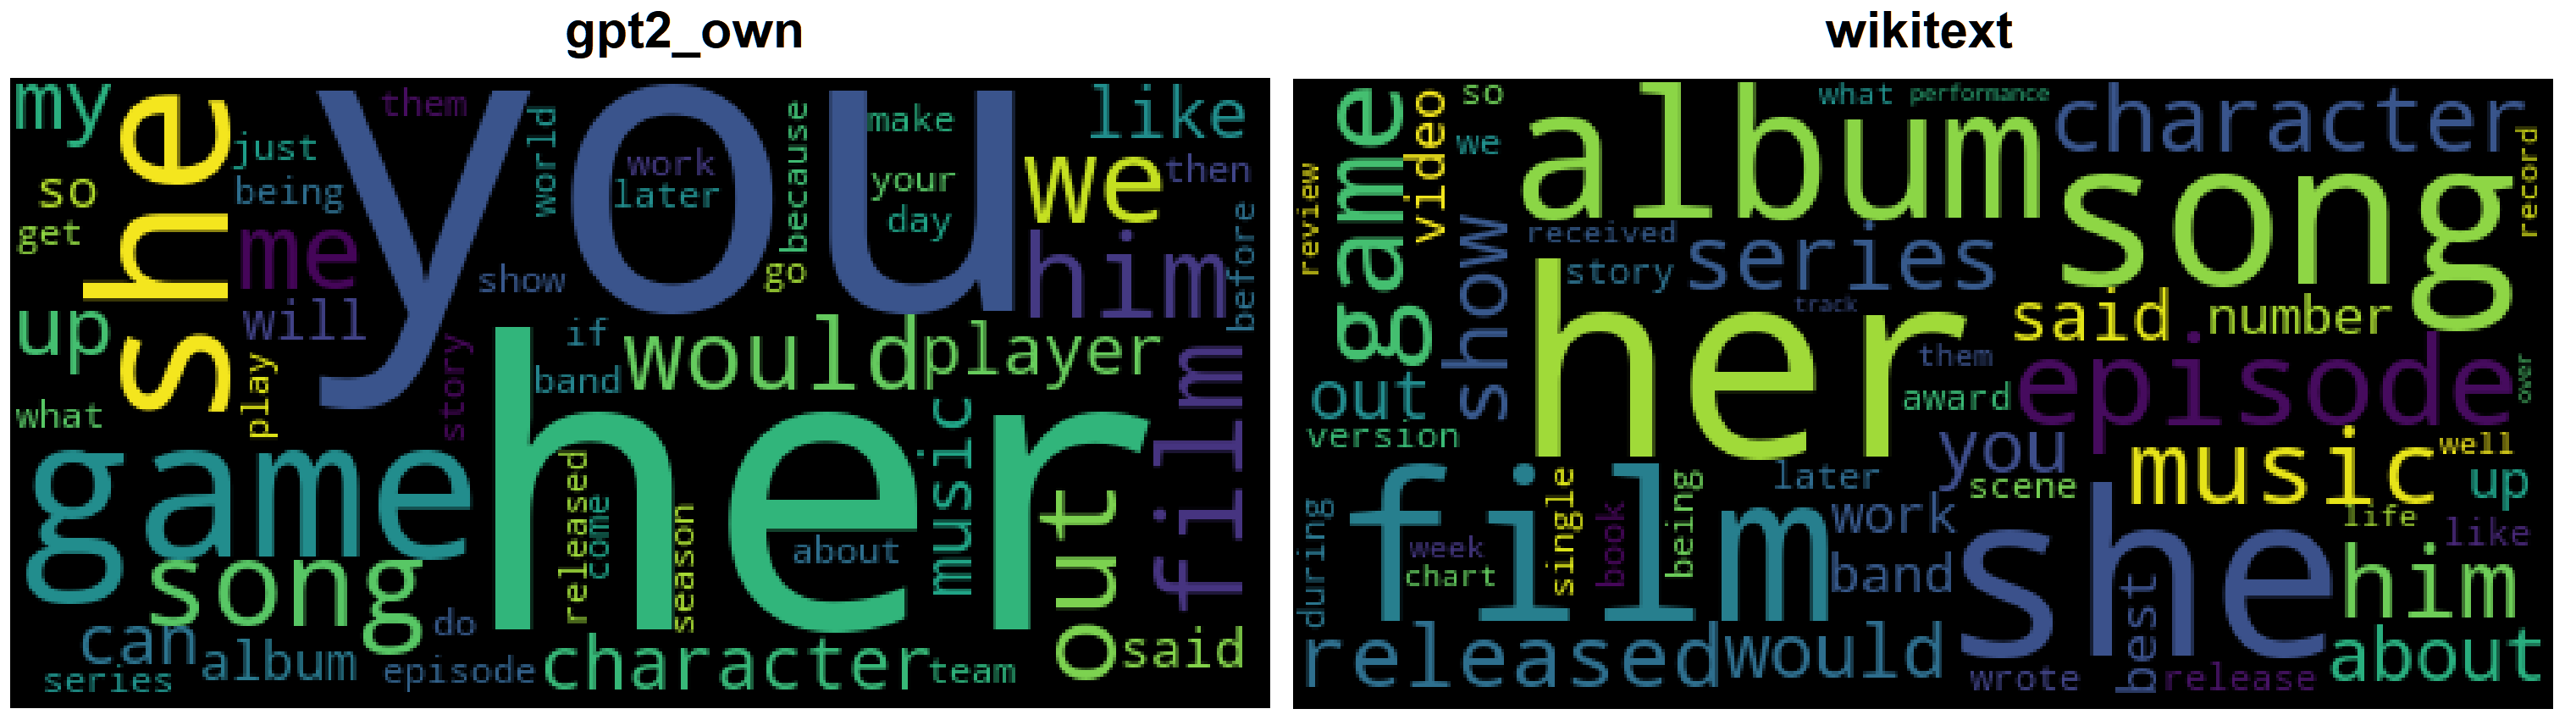
\includegraphics[width=0.8\textwidth]{figures/wordcloud-gpt2_nt-wiki_nt-5-2}
    \caption{Wordcloud example 1 of two similar topics. The size of the word corresponds to the probability of that word in that topic. This is topic 2 out of 5, trained on a corpus with 100'000 documents, using intersected dictionaries and ancestral sampling. Created using classic LDA.}
    \label{fig:wordcloud-gpt2_nt-wiki_nt-5-2}
\end{figure}
\begin{figure}[H]
    \centering
    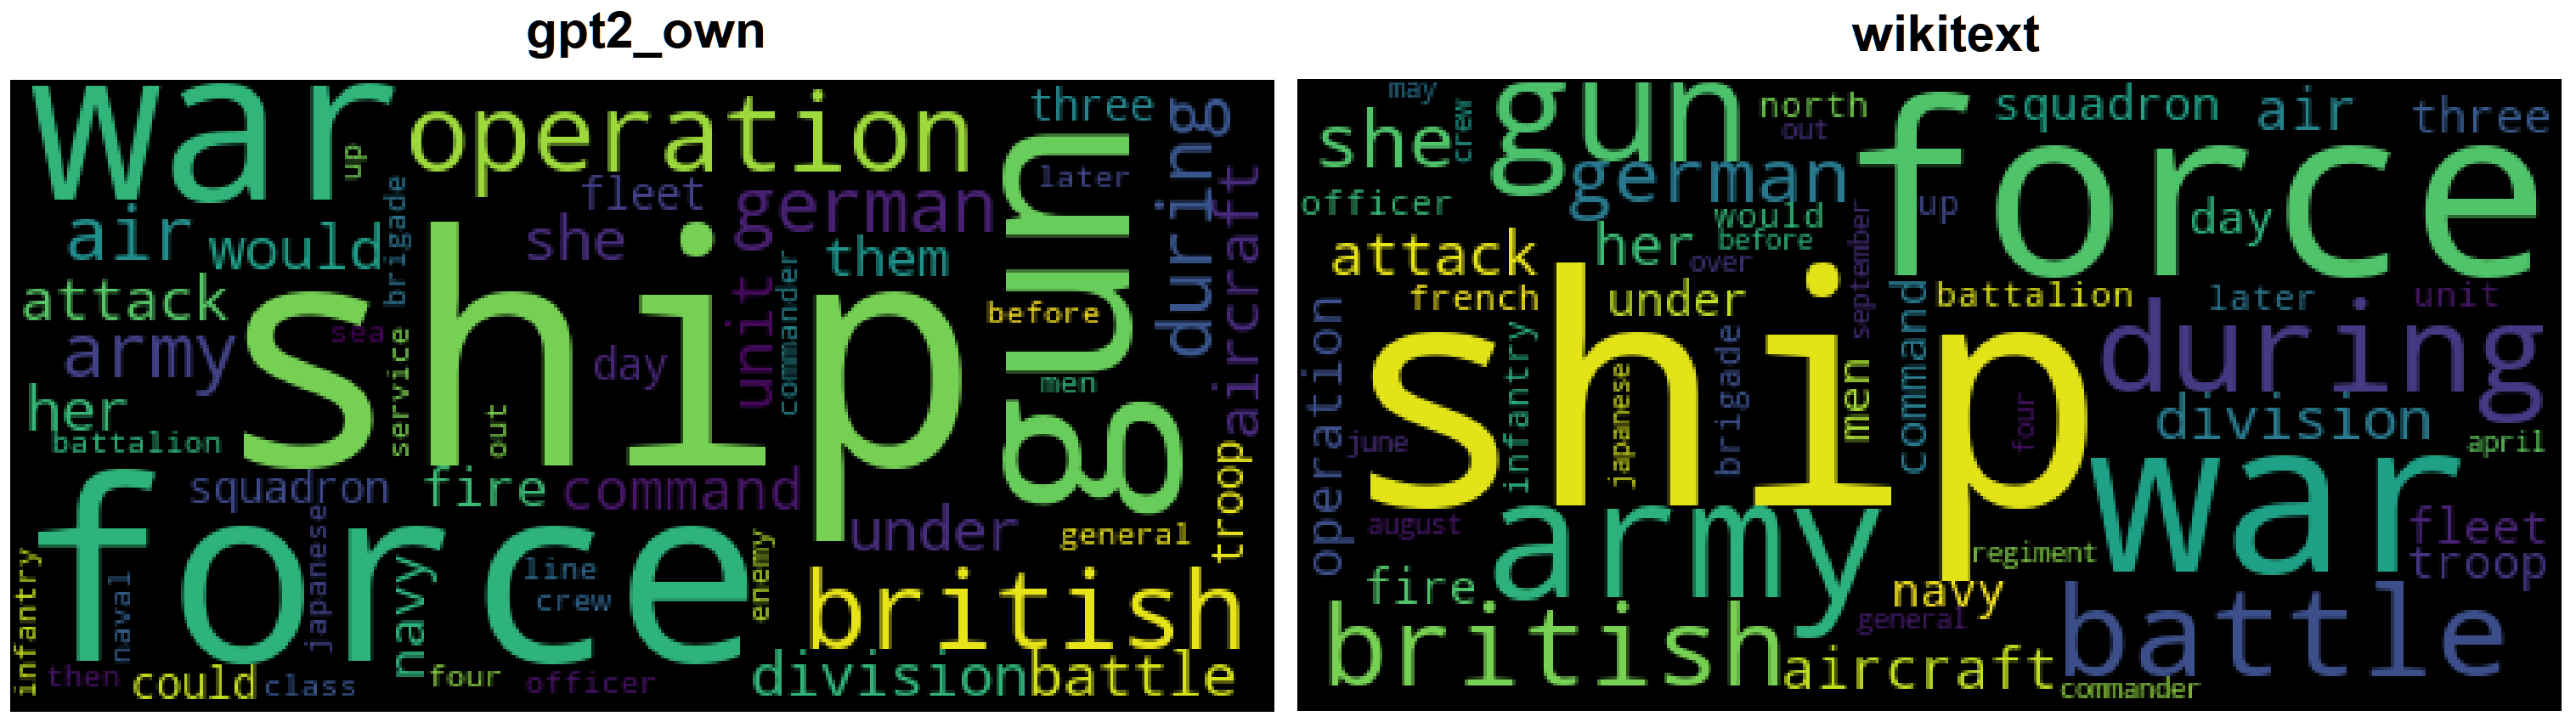
\includegraphics[width=0.8\textwidth]{figures/wordcloud-gpt2_nt-wiki_nt-10-3}
    \caption{Wordcloud example 2 of two similar topics. The size of the word corresponds to the probability of that word in that topic. This is topic 3 out of 10, trained on a corpus with 100'000 documents, using intersected dictionaries and ancestral sampling. Created using classic LDA.}
    \label{fig:wordcloud-gpt2_nt-wiki_nt-10-3}
\end{figure}
To put that comparison into a number, we compare all rows from the topic-word matrices $T_1$ and $T_2$ with each other by using the Jensen-Shannon distance. The rows contain the topic-word distributions of the words. We then obtain two new matrices $M^{(1)}$ and $M^{(2)}$ (see eq. \ref{eq:jsd}) containing those distances for every topic pair.
\begin{equation}\label{eq:jsd}
    \begin{split}
        & M^{(1)}_{i,j}=JSD(P_i||Q_j), \\
        & M^{(2)}_{i,j}=JSD(Q_i||P_j),\\
        & \forall i,j\in[0,n-1],\\
        & n = \text{number of topics,}\\
        & P_i=i-th \text{ row of }T_1,\\
        & Q_j=j-th \text{ row of }T_2
    \end{split}
\end{equation}
Fig. \ref{fig:diff_classic_lda_intersection_5} and \ref{fig:diff_classic_lda_intersection_10} are illustrations of similarity matrices. A deep dark red means that two topics are very different and a deep dark blue indicates the opposite. As shown, not every topic from one model has a matching counterpart. Occasionally, there are multiple topics from the other topic model that are similar to one topic. 
\begin{figure}[H]
    \centering
    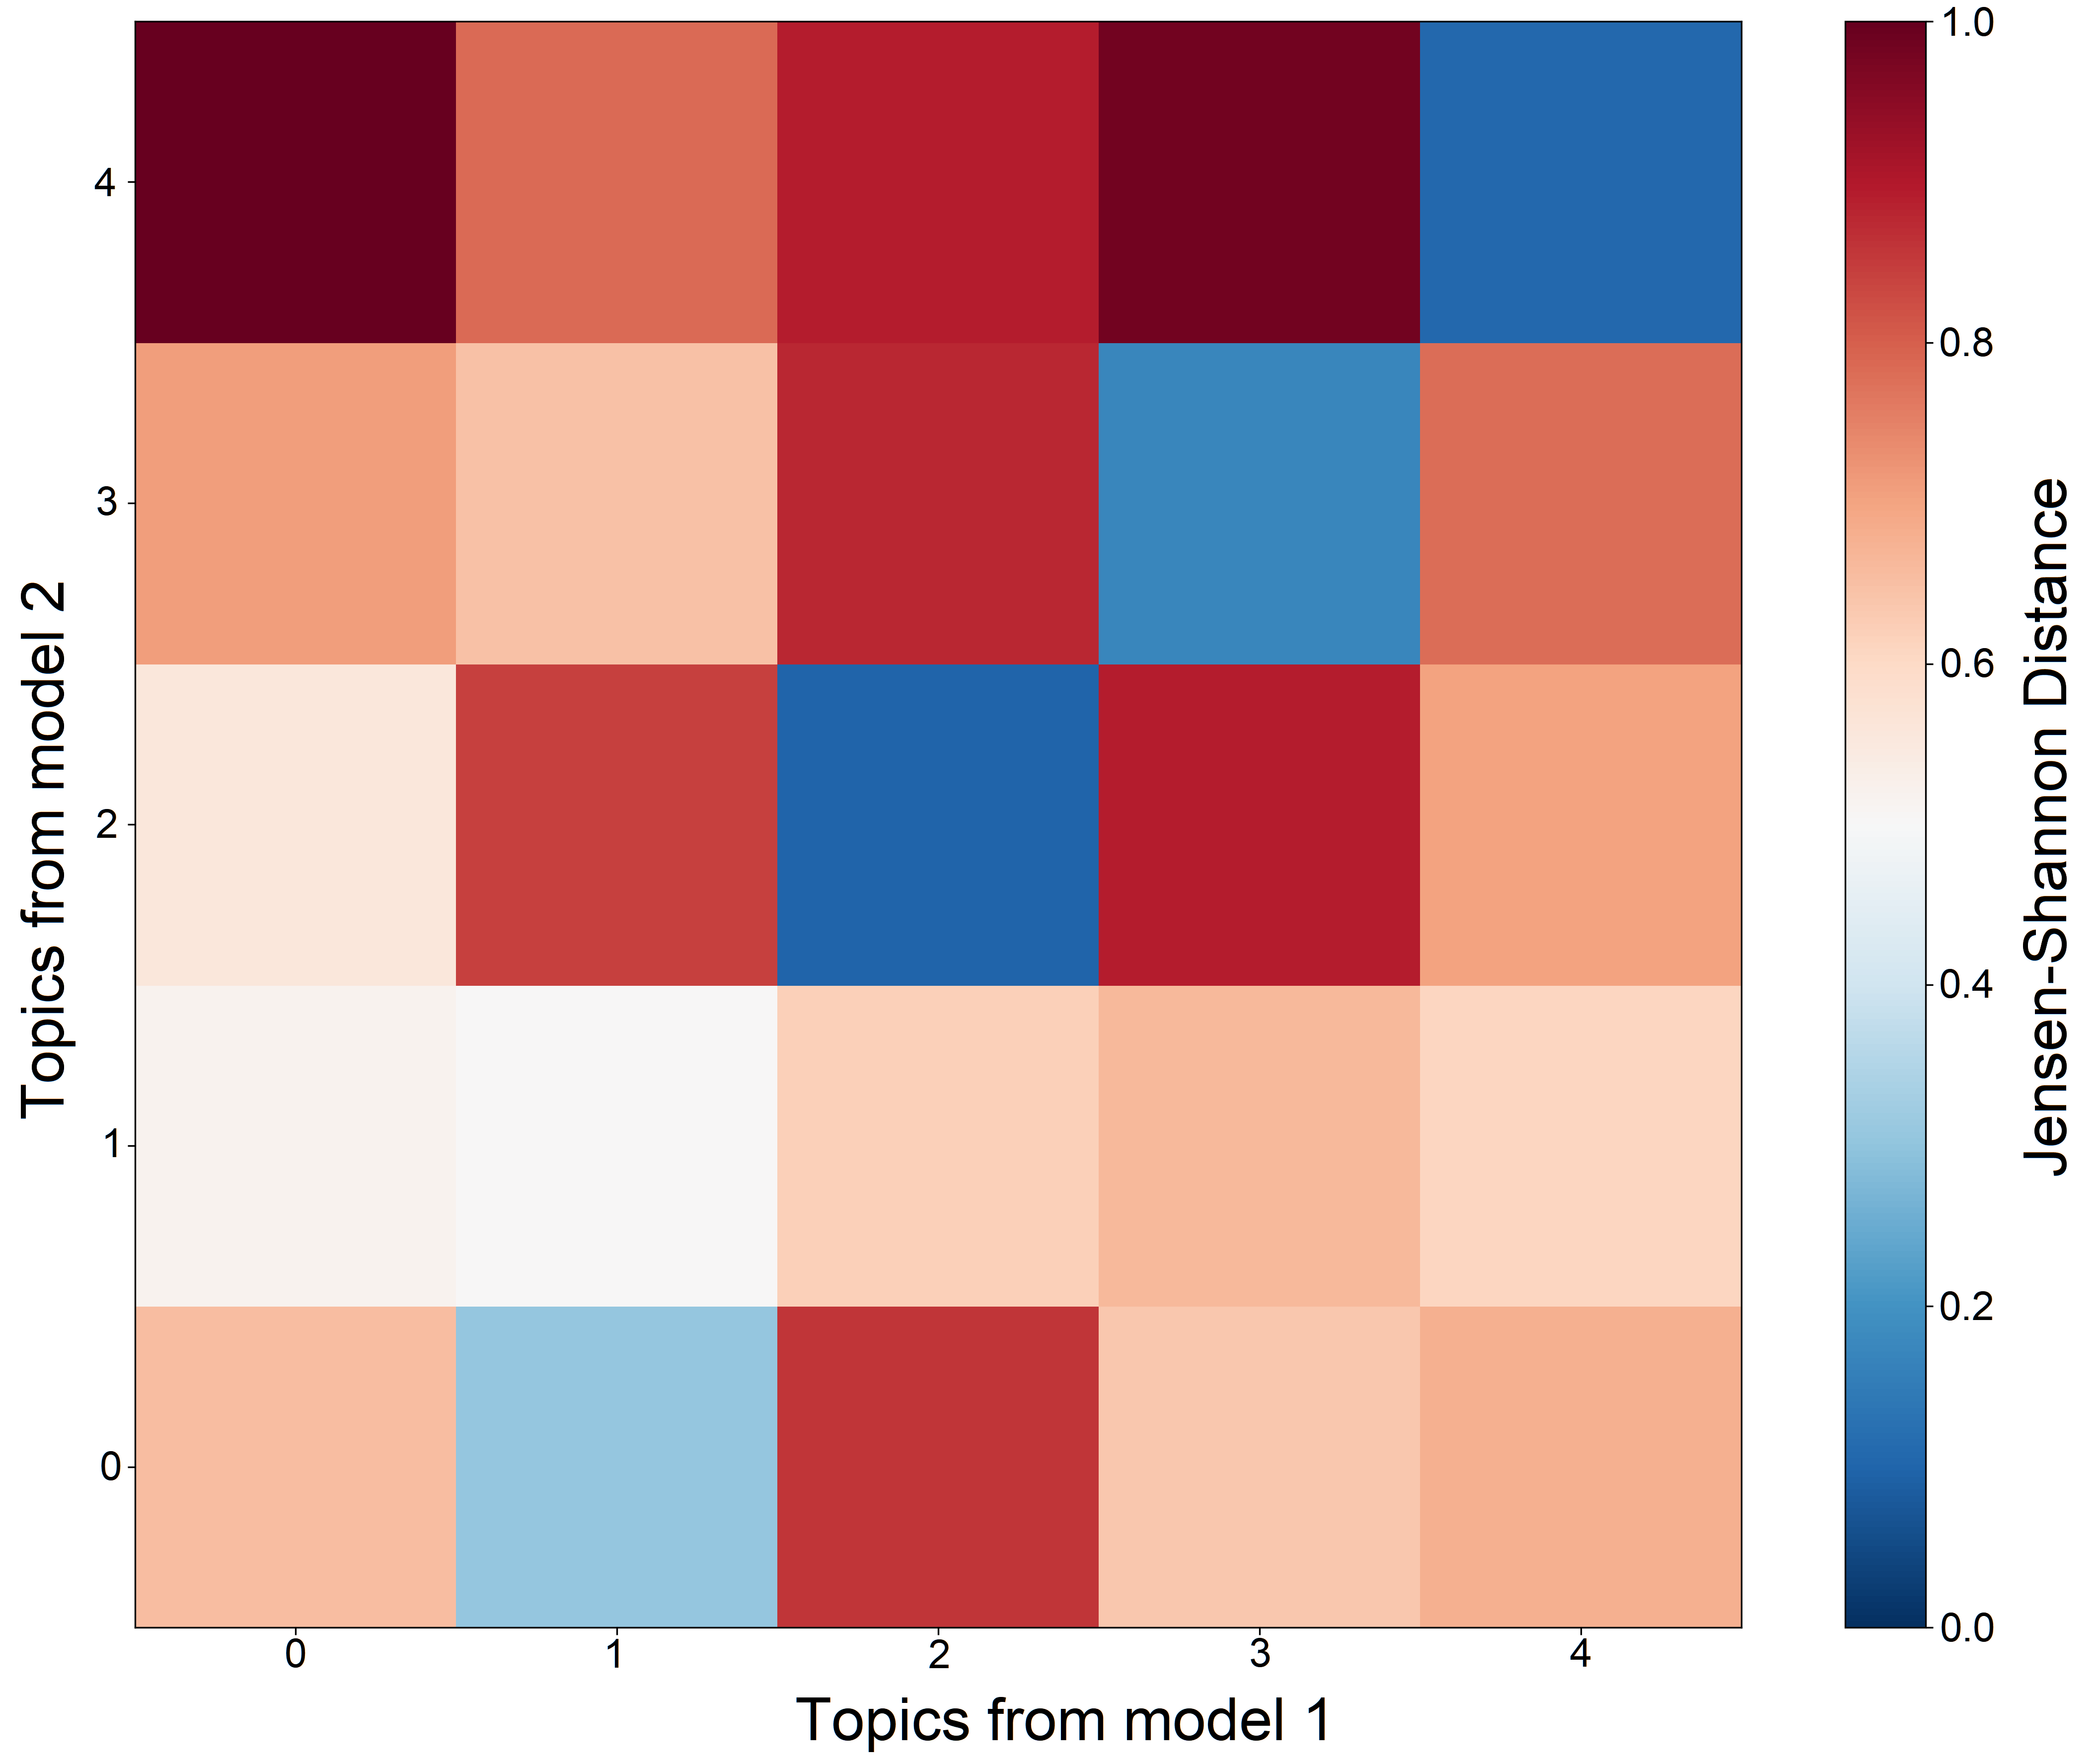
\includegraphics[width=0.5\textwidth]{figures/diff_classic_lda_intersection_5}
    \caption{Illustration of the similarity matrix for 5 topics using the Jensen-Shannon distance. Comparing \texttt{gpt2\_ours} vs. \texttt{wikitext}, trained on a corpus size of 100'000 documents and with intersected dictionaries.}
    \label{fig:diff_classic_lda_intersection_5}
\end{figure}
\begin{figure}[H]
    \centering
    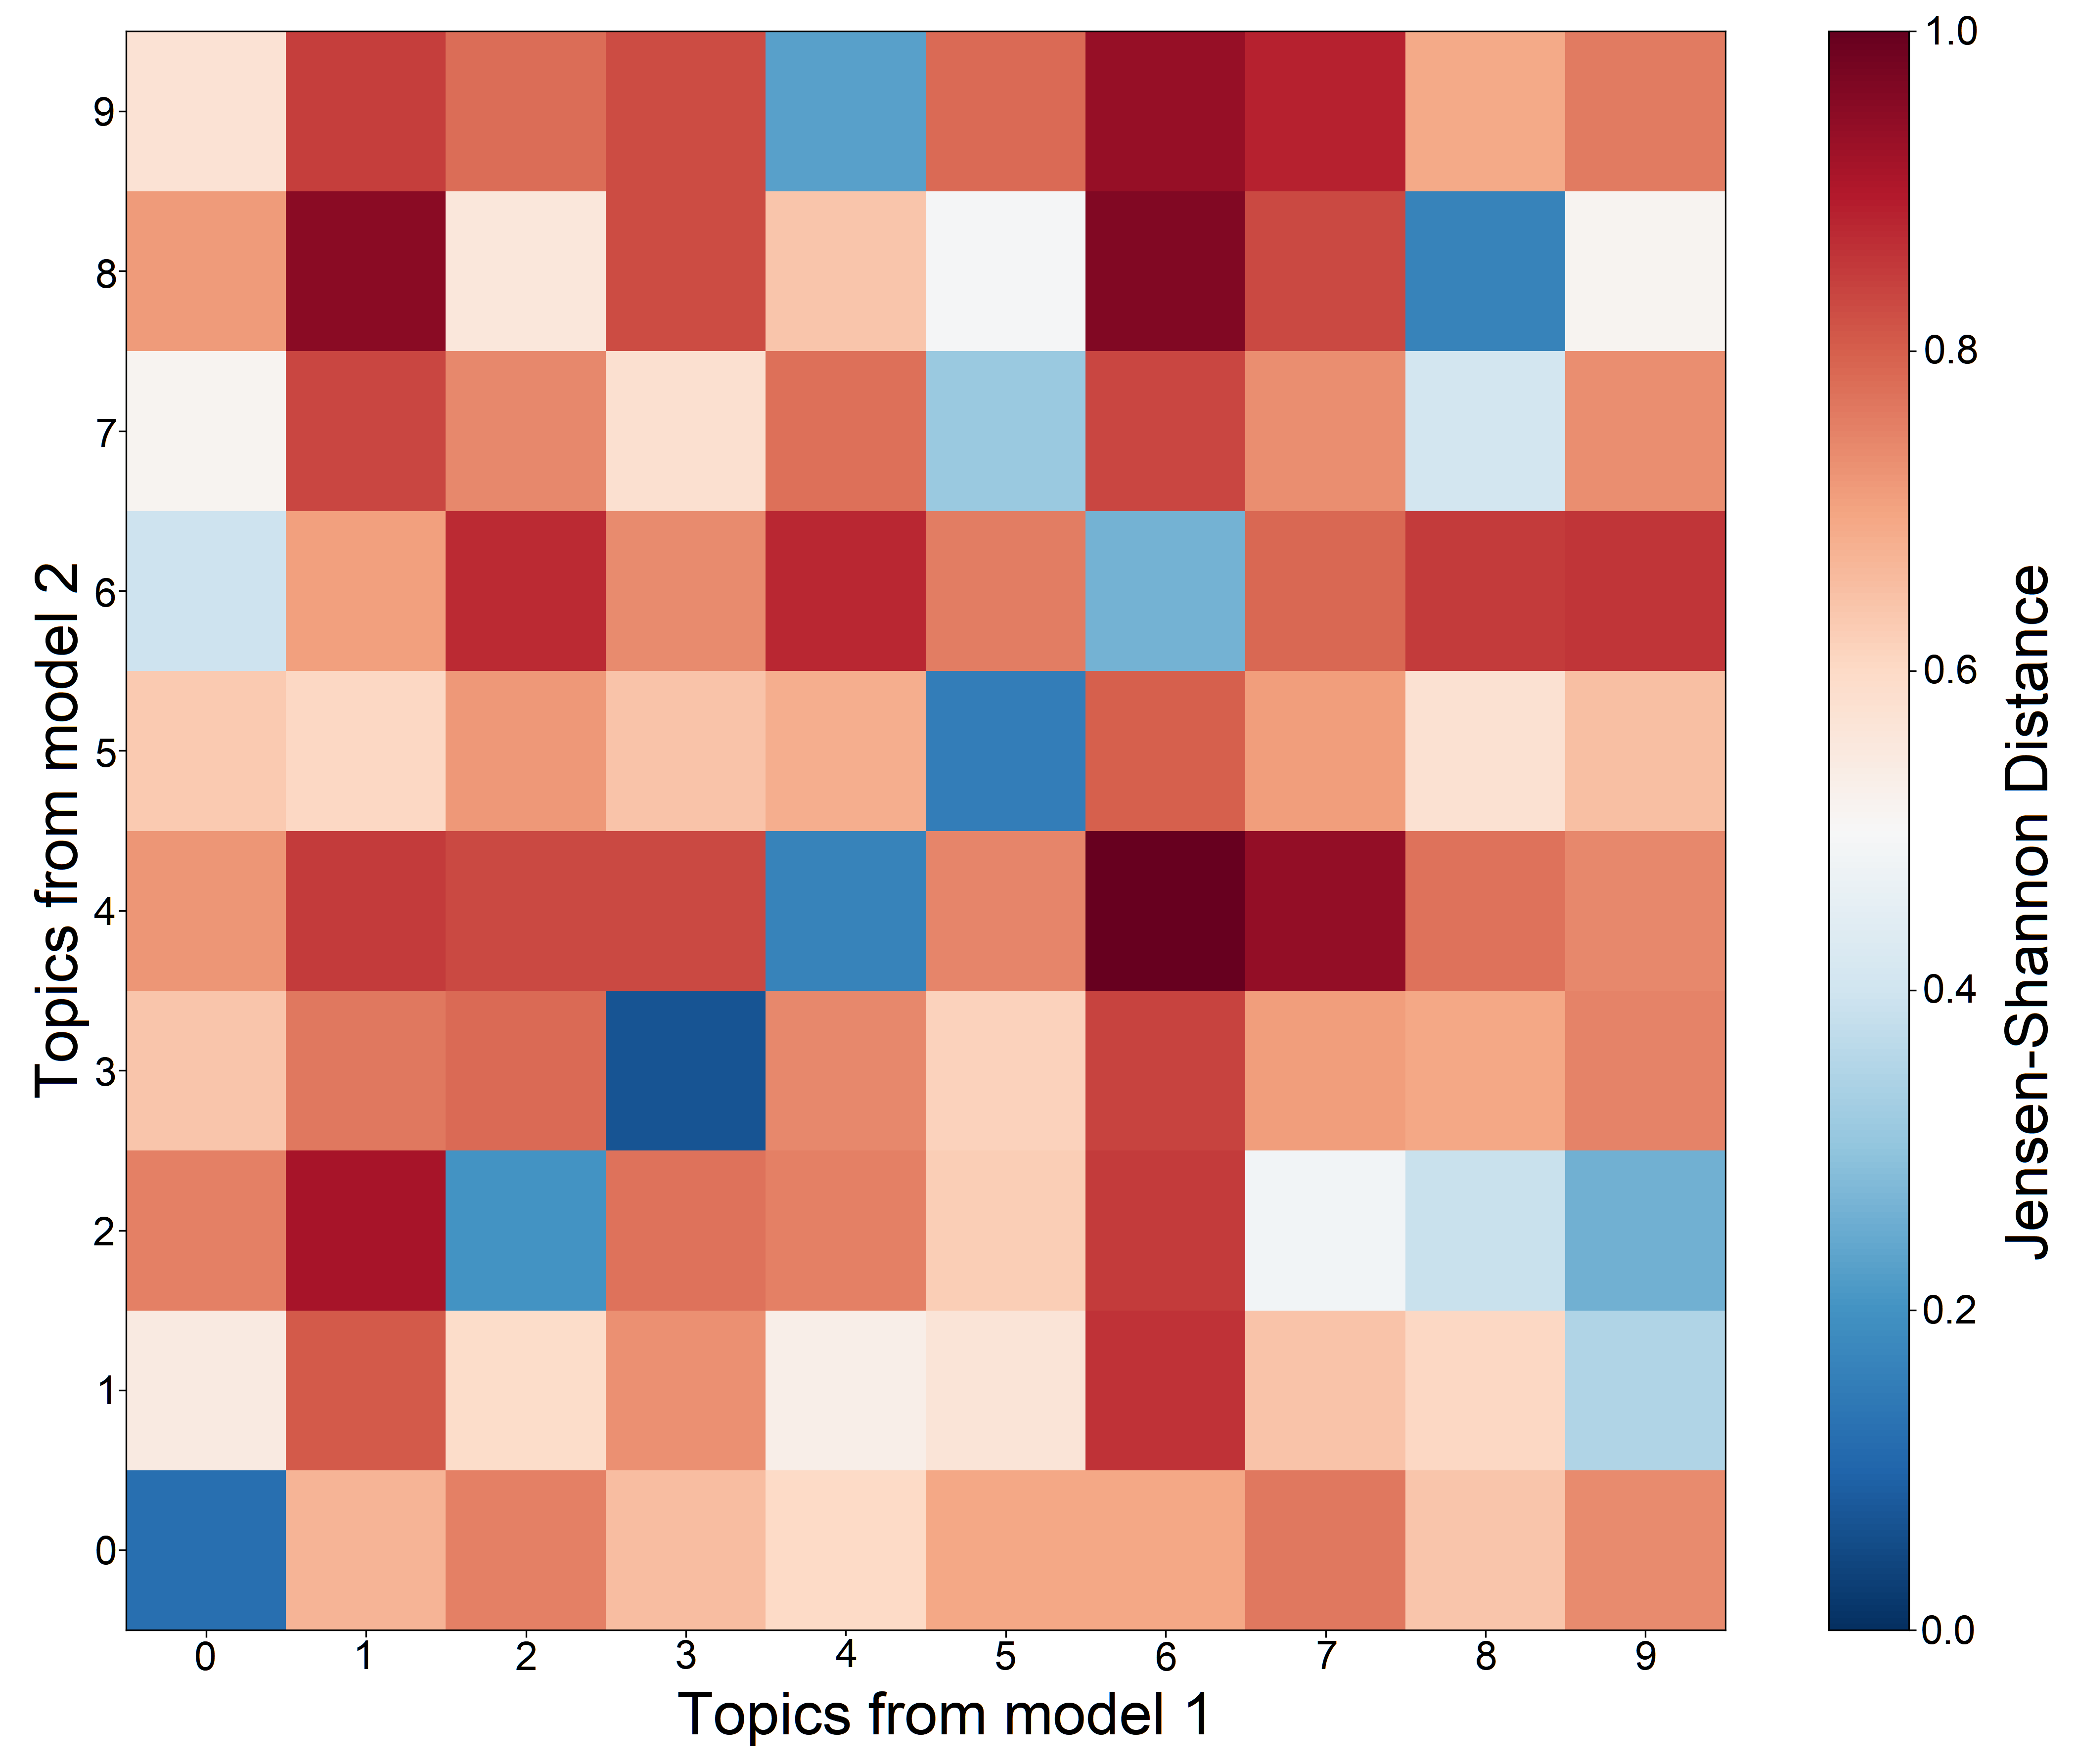
\includegraphics[width=0.6\textwidth]{figures/diff_classic_lda_intersection_10}
    \caption{Illustration of the similarity matrix for 10 topics using the Jensen-Shannon distance. Comparing \texttt{gpt2\_ours} vs. \texttt{wikitext}, trained on a corpus size of 100'000 documents and with intersected dictionaries.}
    \label{fig:diff_classic_lda_intersection_10}
\end{figure}
In order to find out if two topic models found similar clusters, we take the best match for each topic and weigh it by how probable that topic is in the corpus. For this, we calculate the boolean probability of each topic. Meaning, for a topic, we count the number of times it is the most dominant topic in a document, divided by the total number of documents in a corpus. With the two document-topic matrices $D1$ and $D2$, we get the Python code snippet in \ref{eq:probabpython}.
\begin{code}
\captionof{listing}{Topic Probability Calculation}
\label{eq:probabpython}
\begin{minted}{Python}
    import numpy as np
    
    n = number_of_topics
    m = total_numer_of_documents
    u1 = np.argmax(D1, axis=1)  
    u2 = np.argmax(D2, axis=1)
    p1 = np.zeros(n)
    p2 = np.zeros(n)
    
    for topic in range(n):
        p1[topic] = np.count_nonzero(u1 == topic)/m
        p2[topic] = np.count_nonzero(u2 == topic)/m
\end{minted}
\end{code}
Now, we weigh the resulting vector from taking the minimum in every row from the similarity matrix with the probability vector and sum them up. We combine those two operations with the scalar product. Our final metric is the mean of both resulting values as shown in eq. \ref{eq:final}.  
\begin{equation}\label{eq:final}
    \text{metric }=\frac{\langle p1,\text{ amin}(M^{(1)},\text{ axis}=1)\rangle + \langle p2,\text{ amin}(M^{(2)},\text{ axis}=1)\rangle}{2}
\end{equation}

% =======================================
\section{Results}\label{sec:results}
During our experimentation we find that topic models created with intersected dictionaries tend to be more reliable and stable in relation to our metric and the quality of the topic models. We therefore focus our findings on results with intersected dictionaries. Furthermore, we did not find any notable difference in our results by adding bigrams or trigrams to our dictionaries, thus we only report on our findings with unigrams.

% =======================================
\subsection{Quality of Our Language Models}
Concerning the quality of our language models, we do not see a major deviation from the original scores (see table \ref{tab:origcoh}) and can therefore say that the quality of our language models is in the range of confidence of the original scores. This means that we assume our trained language models have learned the language of the corpus they were trained on to the same degree as the original models.
\begin{table}[ht]
\caption{Perplexity}
\centering
    \begin{tabular}{ |p{3cm}||p{3cm}|p{3cm}|  }
        \hline
        Language Model & Original & Ours\\
        \hline
        \hline
        GPT-2          & 37.50 & 32.58\\
        \hline
        Transformer-XL & 24.0  & 27.43\\
        \hline
    \end{tabular}
\label{tab:origcoh}
\end{table}

% =======================================
\subsection{Quality of Our Topic Models}
% =======================================
\subsubsection{Corpora With 100'000 Samples}
For corpora with 100'000 documents, we evaluate the coherence score (mean and variance) in two ways for each corpus (\texttt{gpt2\_ours}, \texttt{gpt2}, \texttt{wikitext}, \texttt{arxiv}). First, we compare the influence of changing the seed when creating a topic model. The mean and variance is taken from topic models with different seeds. As shown in fig. \ref{fig:Unigrams-100000-var-cv-is}, the mean ranges from $0.33$ to $0.58$ and the variance stays in the range of $\pm0.05$ of the mean. On average, we can see that the quality of each of our topic models here is the highest when using $20$ to $50$ topics.
\begin{figure}[H]
    \centering
    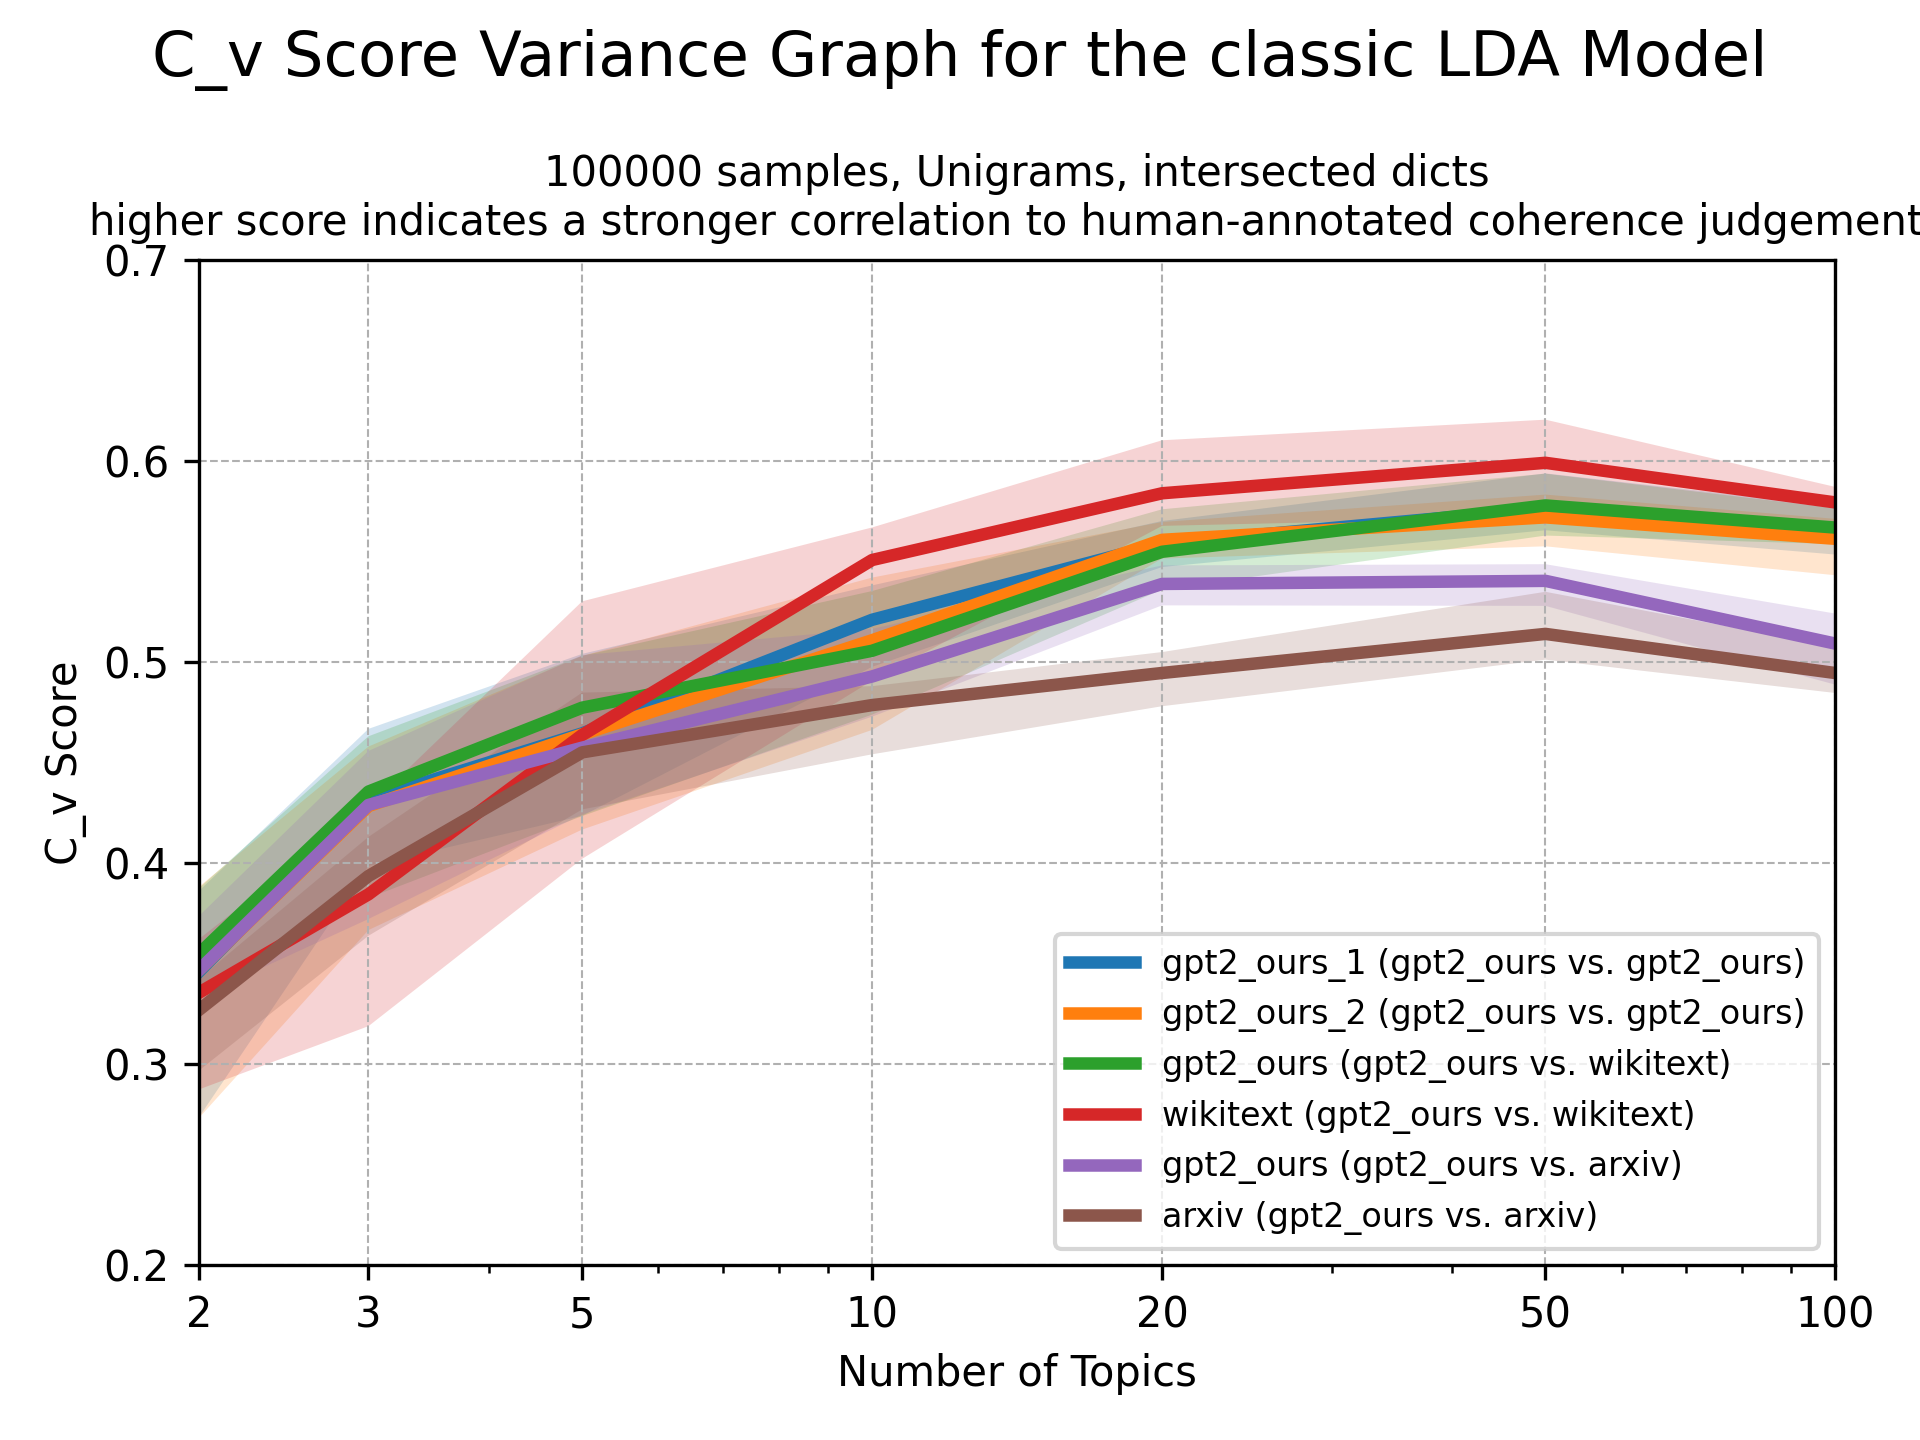
\includegraphics[width=0.6\textwidth]{figures/Unigrams-100000-var-cv-is}
    \caption{Topic coherence of topic models with different seed.}
    \label{fig:Unigrams-100000-var-cv-is}
\end{figure}
Secondly, we compare the influence of a slightly changed dictionary. As previously mentioned, we take the intersection of each dictionary pair of which we want to compare the corpora. This means, when looking at the \texttt{wikitext} corpus, we get 7 different dictionaries and therefore 7 slightly different topic models for that corpus. Those different dictionaries result from comparing the corpus with \texttt{gpt2}, \texttt{arxiv}, \texttt{gpt\_ours}, \texttt{gpt\_ours} with Top-P sampling, \texttt{gpt\_ours} with Typical sampling and twice for \texttt{wikitext} itself. As shown in fig. \ref{fig:Unigrams-100000-crossmodel-cv-var-classic_lda-gpt2+nt-is} on the left, the topic model scores are in a similar range of $0.29$ to $0.59$ with a variance of $\pm0.05$. On average, we can see that the quality of each of our topic models here is the highest when using $20$ to $50$ topics. 

We also evaluate the influence of different sampling methods for the \texttt{gpt2\_own} corpus and the quality of the resulting topic models. Fig. \ref{fig:Unigrams-100000-crossmodel-cv-var-classic_lda-gpt2+nt-is} on the right shows that on average Top-P and even more so Typical sampling improves the quality of topics created by topic models.
\begin{figure}[H]
    \centering
    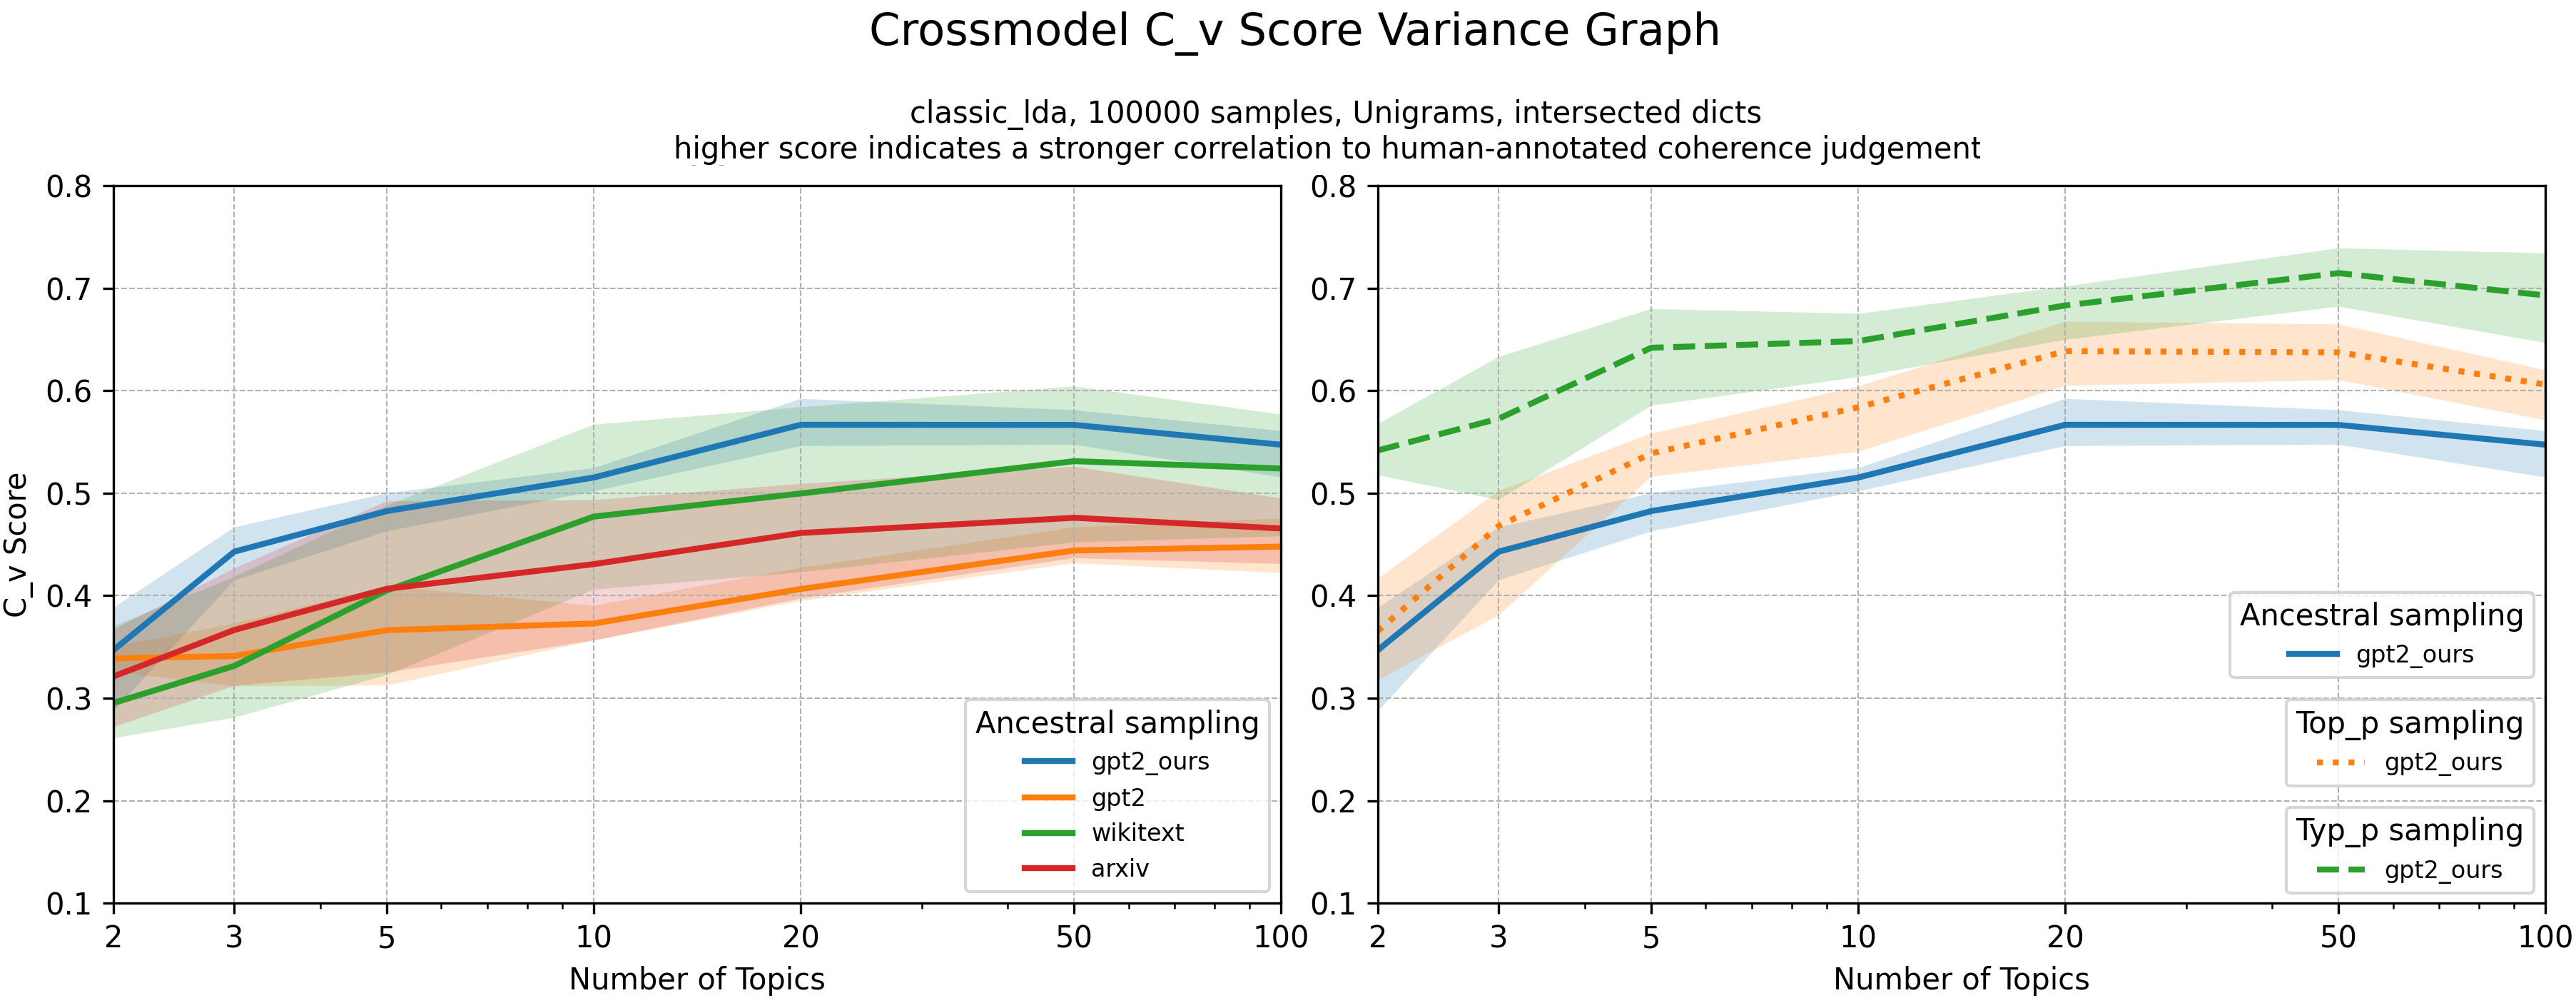
\includegraphics[width=1\textwidth]{figures/Unigrams-100000-crossmodel-cv-var-classic_lda-gpt2+nt-is}
    \caption{Topic coherence of topic models with slightly different dictionaries.}
    \label{fig:Unigrams-100000-crossmodel-cv-var-classic_lda-gpt2+nt-is}
\end{figure}

% =======================================
\subsubsection{Corpora With 10'000 Samples}
Similar to corpora with 100'000 documents, for corpora with 10'000 documents, we first compare the influence of changing the seed when creating a topic model. The mean and variance is taken from topic models with different seeds. In fig. \ref{fig:Unigrams-10000-var-cv-is}, the mean ranges from $0.31$ to $0.58$ and the variance stays in range of $\pm0.05$ of the mean. On average, we see that the quality of each of our topic models here is the highest when using $10$ to $50$ topics, depending on the corpus. 
\begin{figure}[H]
    \centering
    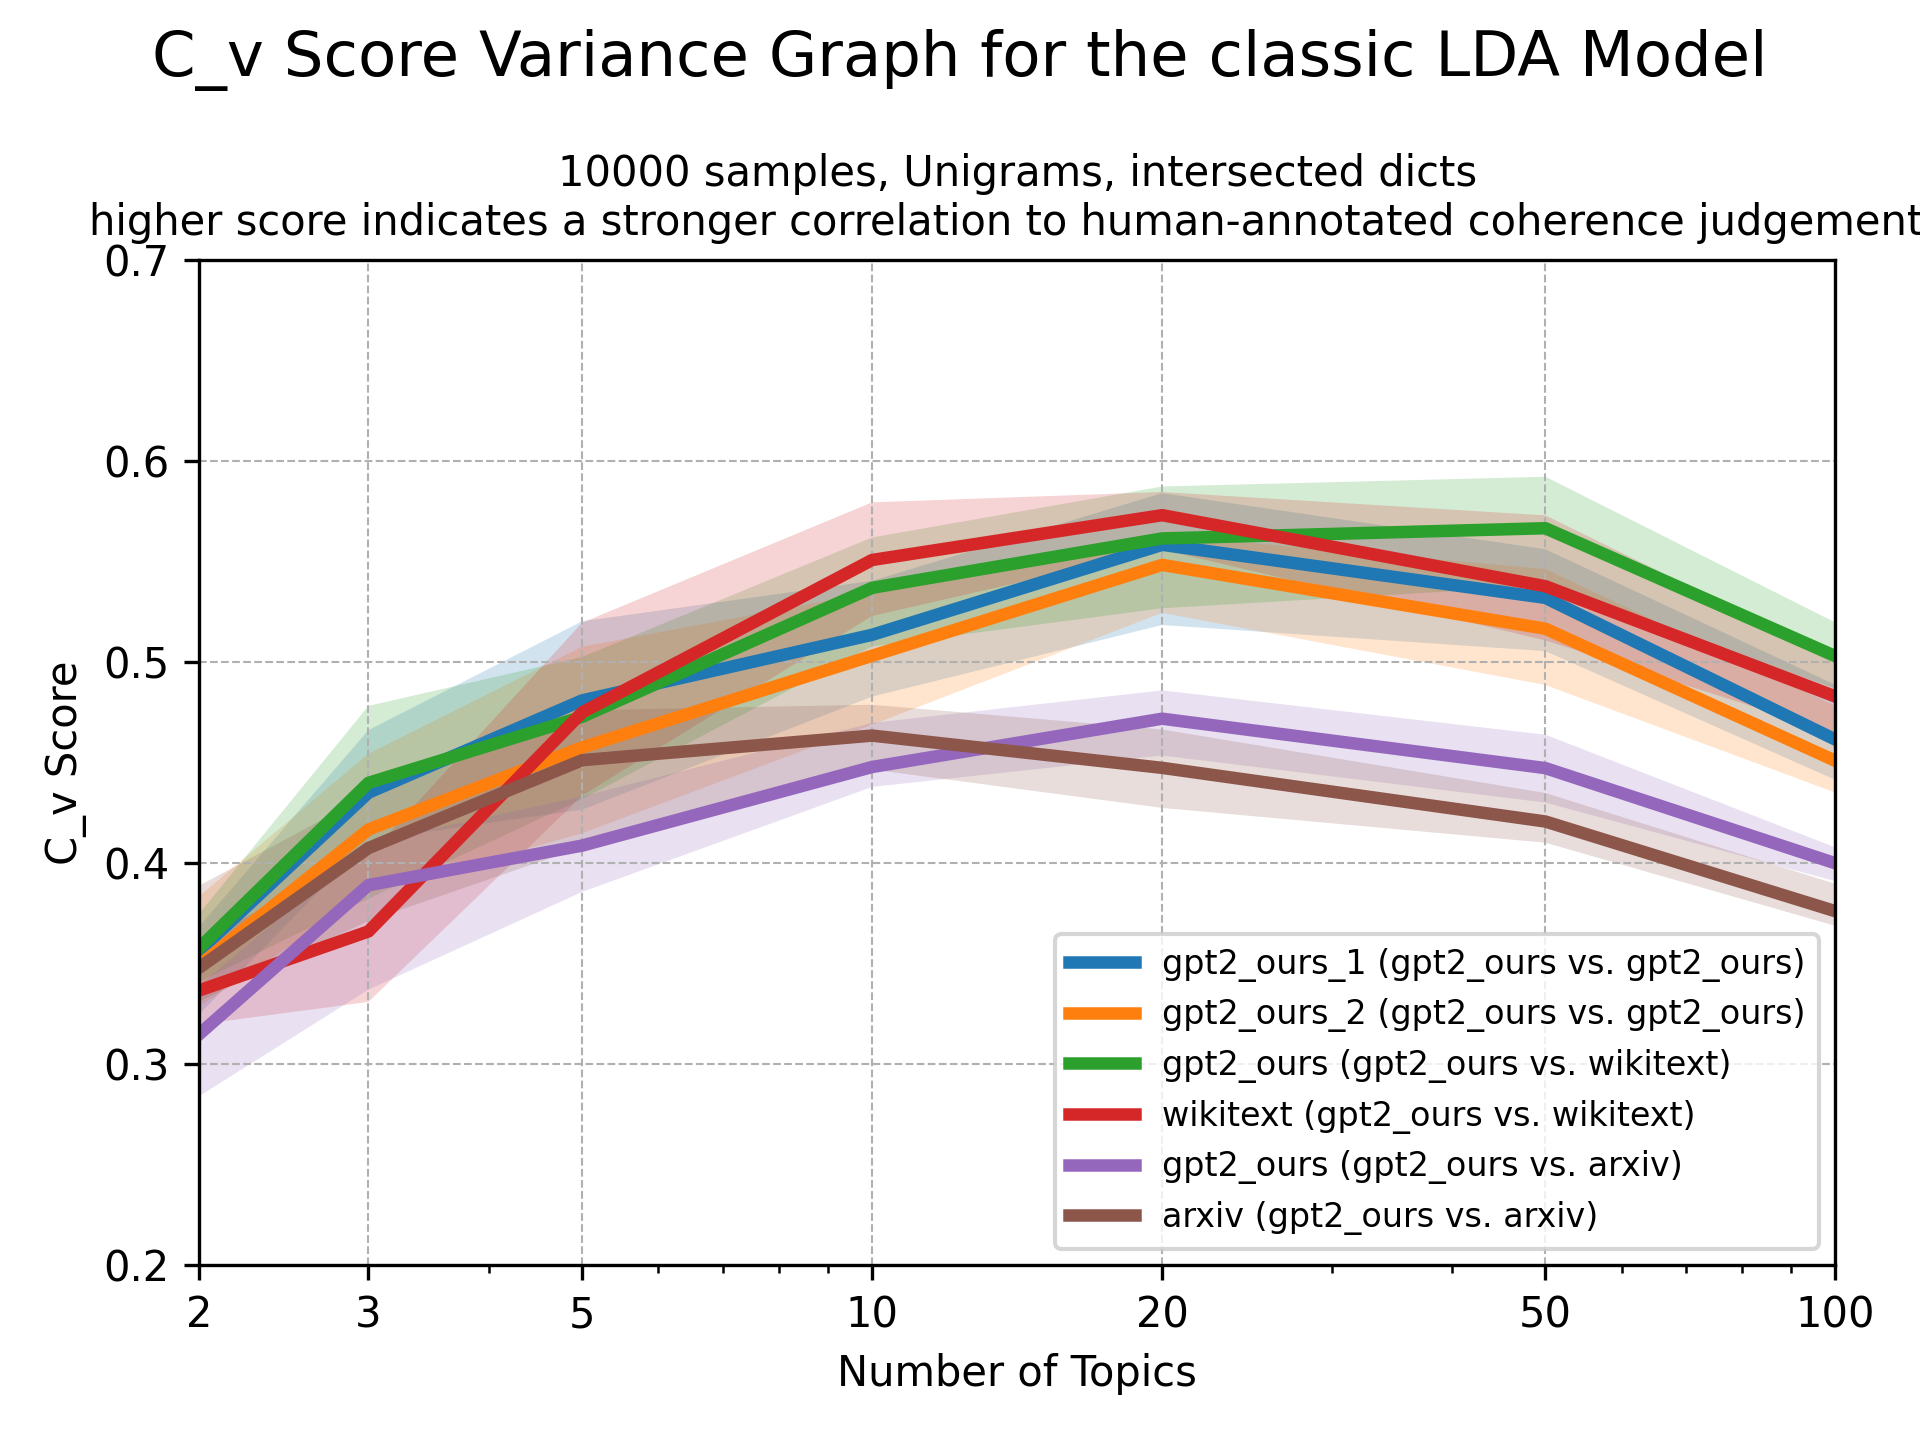
\includegraphics[width=0.6\textwidth]{figures/Unigrams-10000-var-cv-is}
    \caption{Topic coherence of topic models with changing seed.}
    \label{fig:Unigrams-10000-var-cv-is}
\end{figure}
We also compare the effect of a slightly changed dictionary. In contrast to 100'000 samples, we now have additional topic models. We add the evaluation of topic models created with the neural LDA and from additional corpora, i.e. \texttt{trafo\_xl}, \texttt{trafo\_xl\_own}, \texttt{trafo\_xl\_own} sampled with Top-P sampling and \texttt{trafo\_xl\_own} sampled with Typical sampling. With this, we get 11 topic models for the \texttt{wikitext} corpus with a (slightly) different dictionary. 

% =======================================
\subsubsection{GPT-2 With Classic LDA}
Fig. \ref{fig:Unigrams-10000-crossmodel-cv-var-classic_lda-gpt2+nt-is} on the left shows the results in respect to the GPT-2 models. The topic model scores are in a range of $0.31$ to $0.53$ with a variance of $\pm0.05$. On average, we can see that the quality of each of our topic models here is the highest when using $5$ to $20$ topics, depending on the corpus.

Fig. \ref{fig:Unigrams-10000-crossmodel-cv-var-classic_lda-gpt2+nt-is} on the right shows the influence of different sampling methods for the \texttt{gpt2\_own} corpus. On average, Top-P and even more Typical sampling improve the quality of topics created by topic models.
\begin{figure}[H]
    \centering
    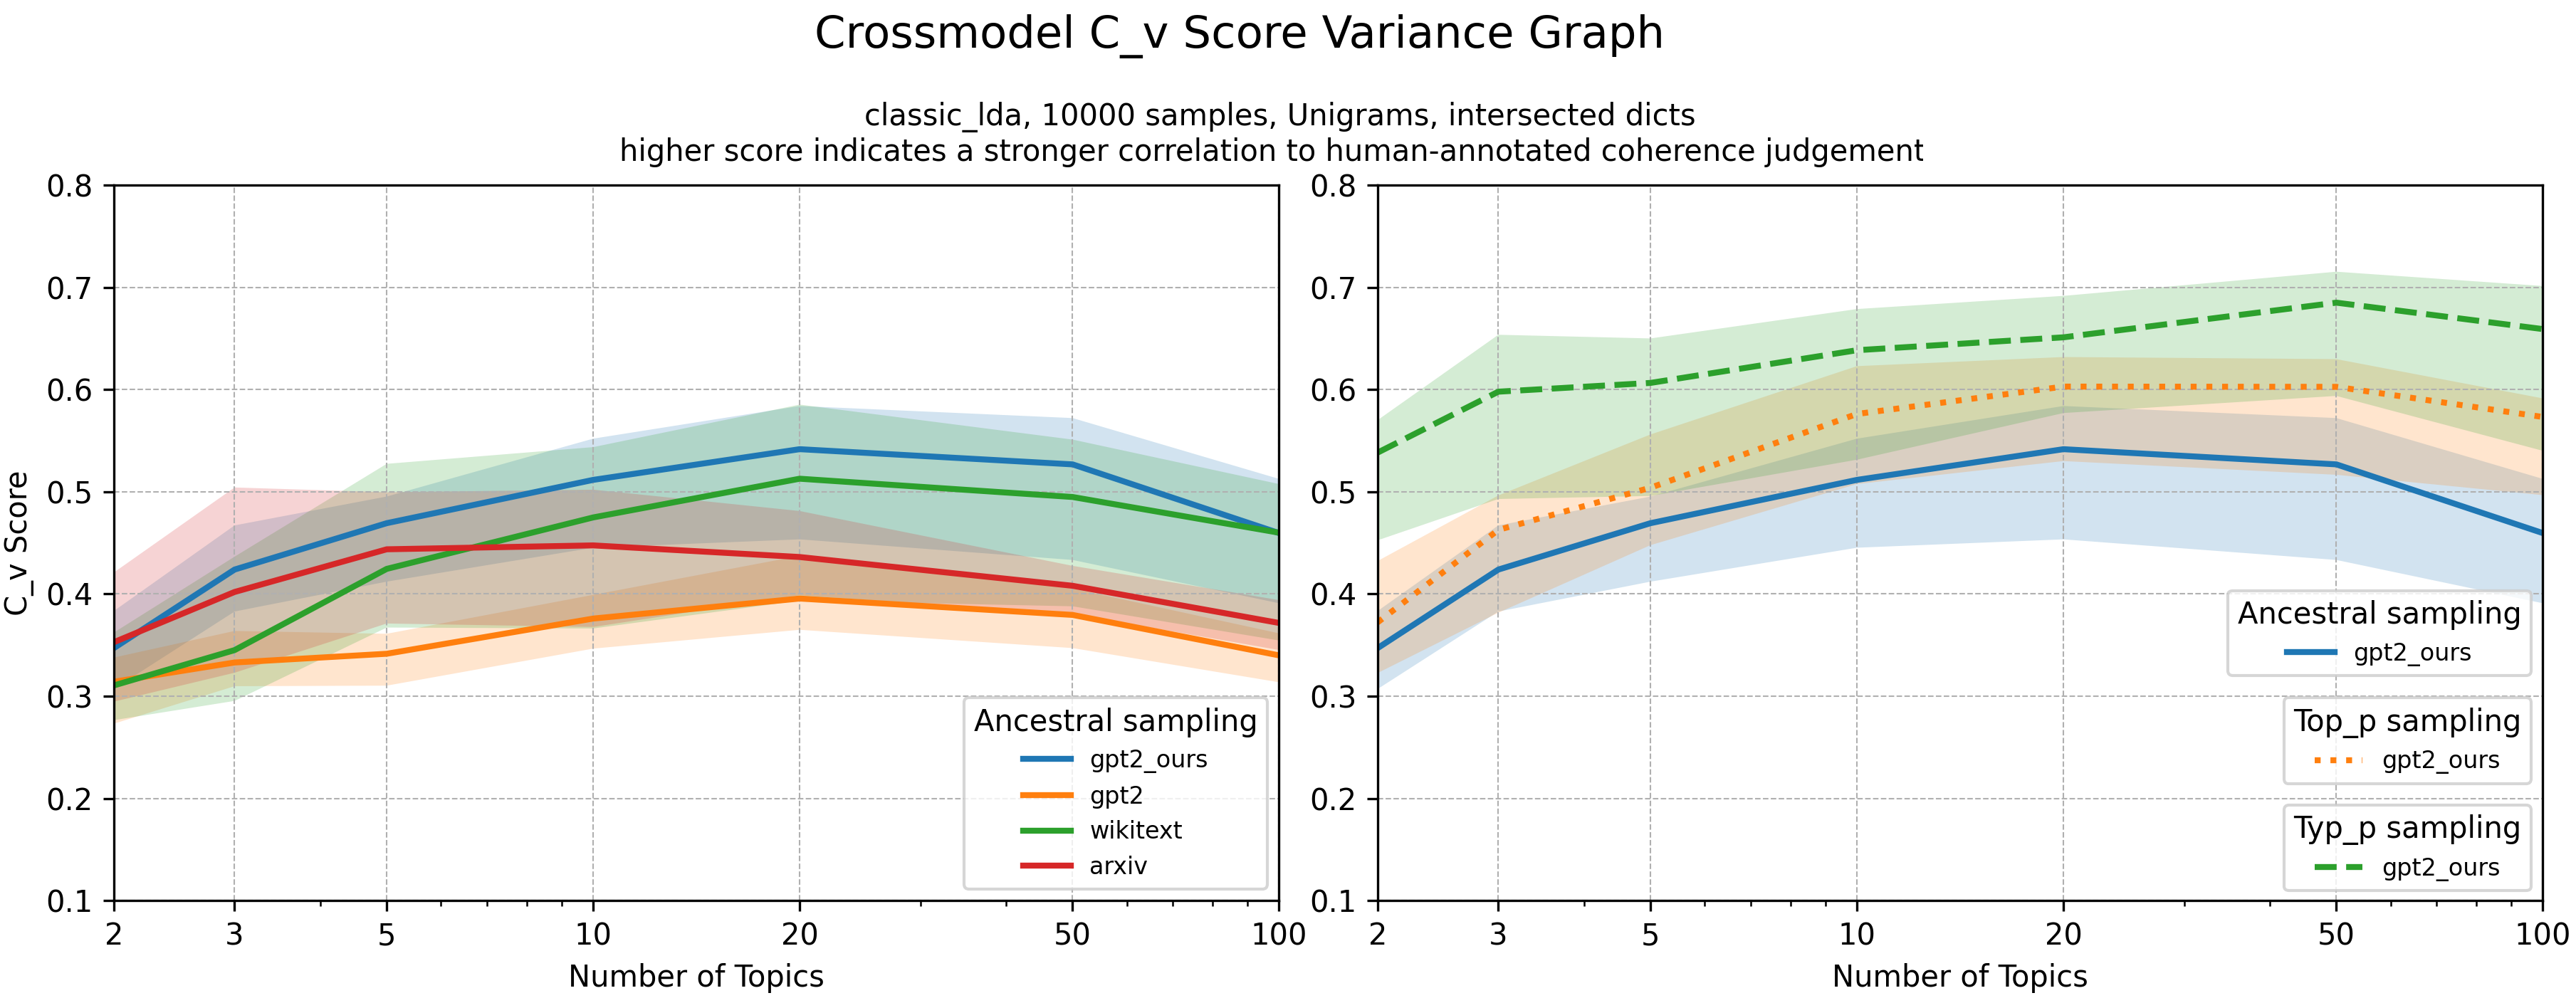
\includegraphics[width=1\textwidth]{figures/Unigrams-10000-crossmodel-cv-var-classic_lda-gpt2+nt-is}
    \caption{Topic coherence of topic models with slightly different dictionaries.}
    \label{fig:Unigrams-10000-crossmodel-cv-var-classic_lda-gpt2+nt-is}
\end{figure}

% =======================================
\subsubsection{Transformer-XL With Classic LDA}
Fig. \ref{fig:Unigrams-10000-crossmodel-cv-var-classic_lda-trafo_xl+nt-is} on the left shows our results with classic LDA in reference to the Tranformer-XL models. The topic model scores are in a range of $0.31$ to $0.56$ with a variance of $\pm0.1$. On average, we see that the quality of our topic models is the highest when using $5$ to $20$ topics, depending on the corpus.

In fig. \ref{fig:Unigrams-10000-crossmodel-cv-var-classic_lda-trafo_xl+nt-is} on the right, we see that for a lower number of topics (2 to 10), different sampling methods do not make a notable difference. For topic models with a topic count of 10 or more Top-P and even more Typical sampling leads to better topic models than ancestral sampling.
\begin{figure}[H]
    \centering
    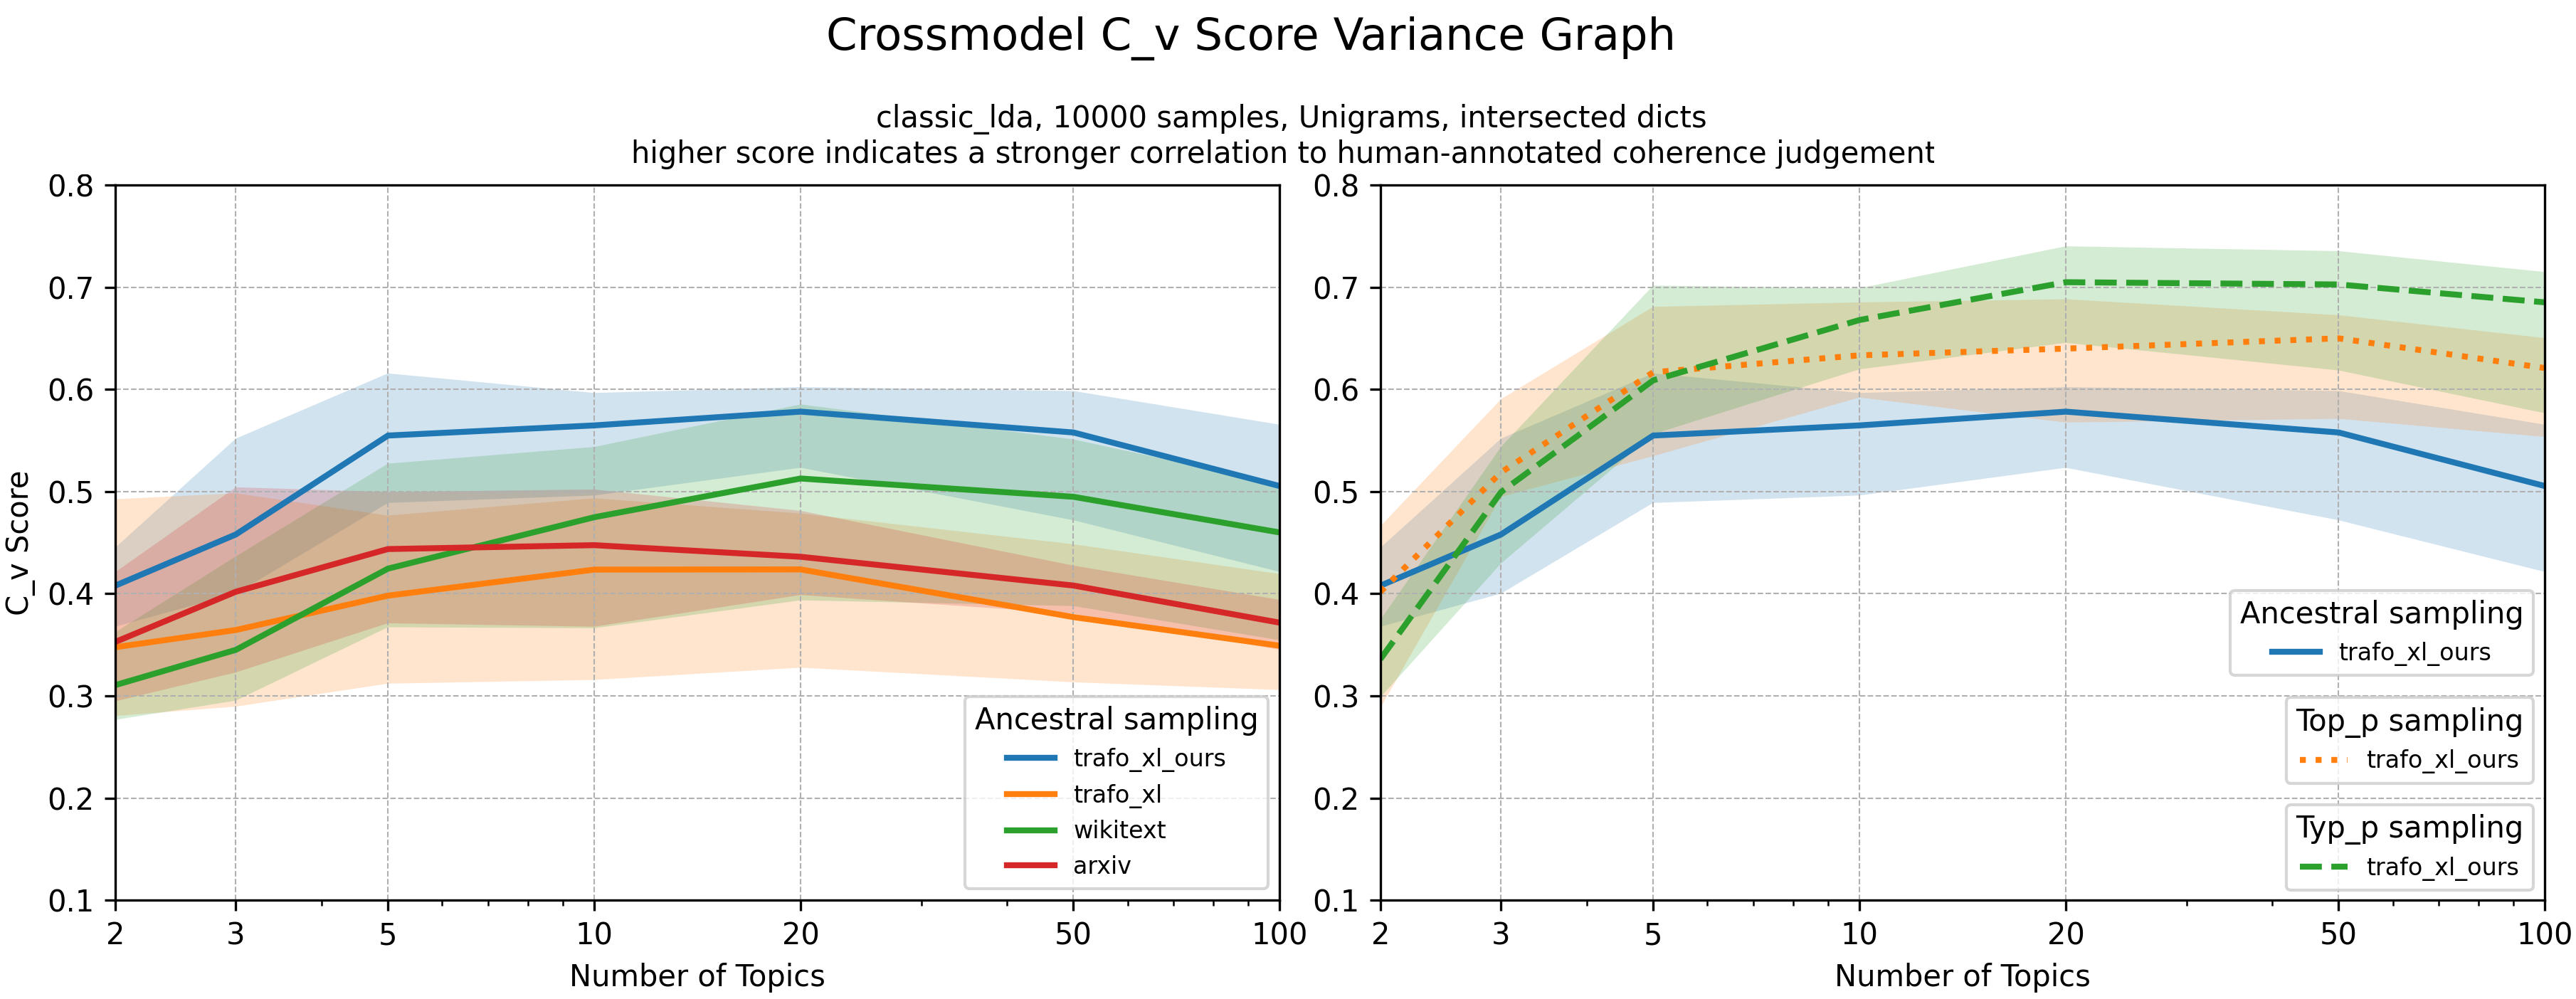
\includegraphics[width=1\textwidth]{figures/Unigrams-10000-crossmodel-cv-var-classic_lda-trafo_xl+nt-is}
    \caption{Topic coherence of topic models with slightly different dictionaries.}
    \label{fig:Unigrams-10000-crossmodel-cv-var-classic_lda-trafo_xl+nt-is}
\end{figure}

% =======================================
\subsubsection{GPT-2 With Neural LDA}
Fig. \ref{fig:Unigrams-10000-crossmodel-cv-var-neural_lda-gpt2+nt-is} shows the quality of topic models created with neural LDA in respect to GPT-2 models. Interestingly, the inverse peak is at 3 topics. All topic models created with neural LDA have this in common. After 5 topics, the scores range from $0.3$ to $0.45$ with a variance of up to $\pm0.1$. The quality with 5 topics or more is approximately horizontal and definitely worse than with the classic LDA. 

The influence of different sampling methods for the \texttt{gpt2\_own} corpus and the quality of the resulting topic models is shown in fig. \ref{fig:Unigrams-10000-crossmodel-cv-var-neural_lda-gpt2+nt-is}. Note that by changing the sampling method, the inverse peak observed with ancestral sampling at 3 topics gets smoothed out. On average, Top-P and even more Typical sampling improve the quality of topics created by topic models.
\begin{figure}[H]
    \centering
    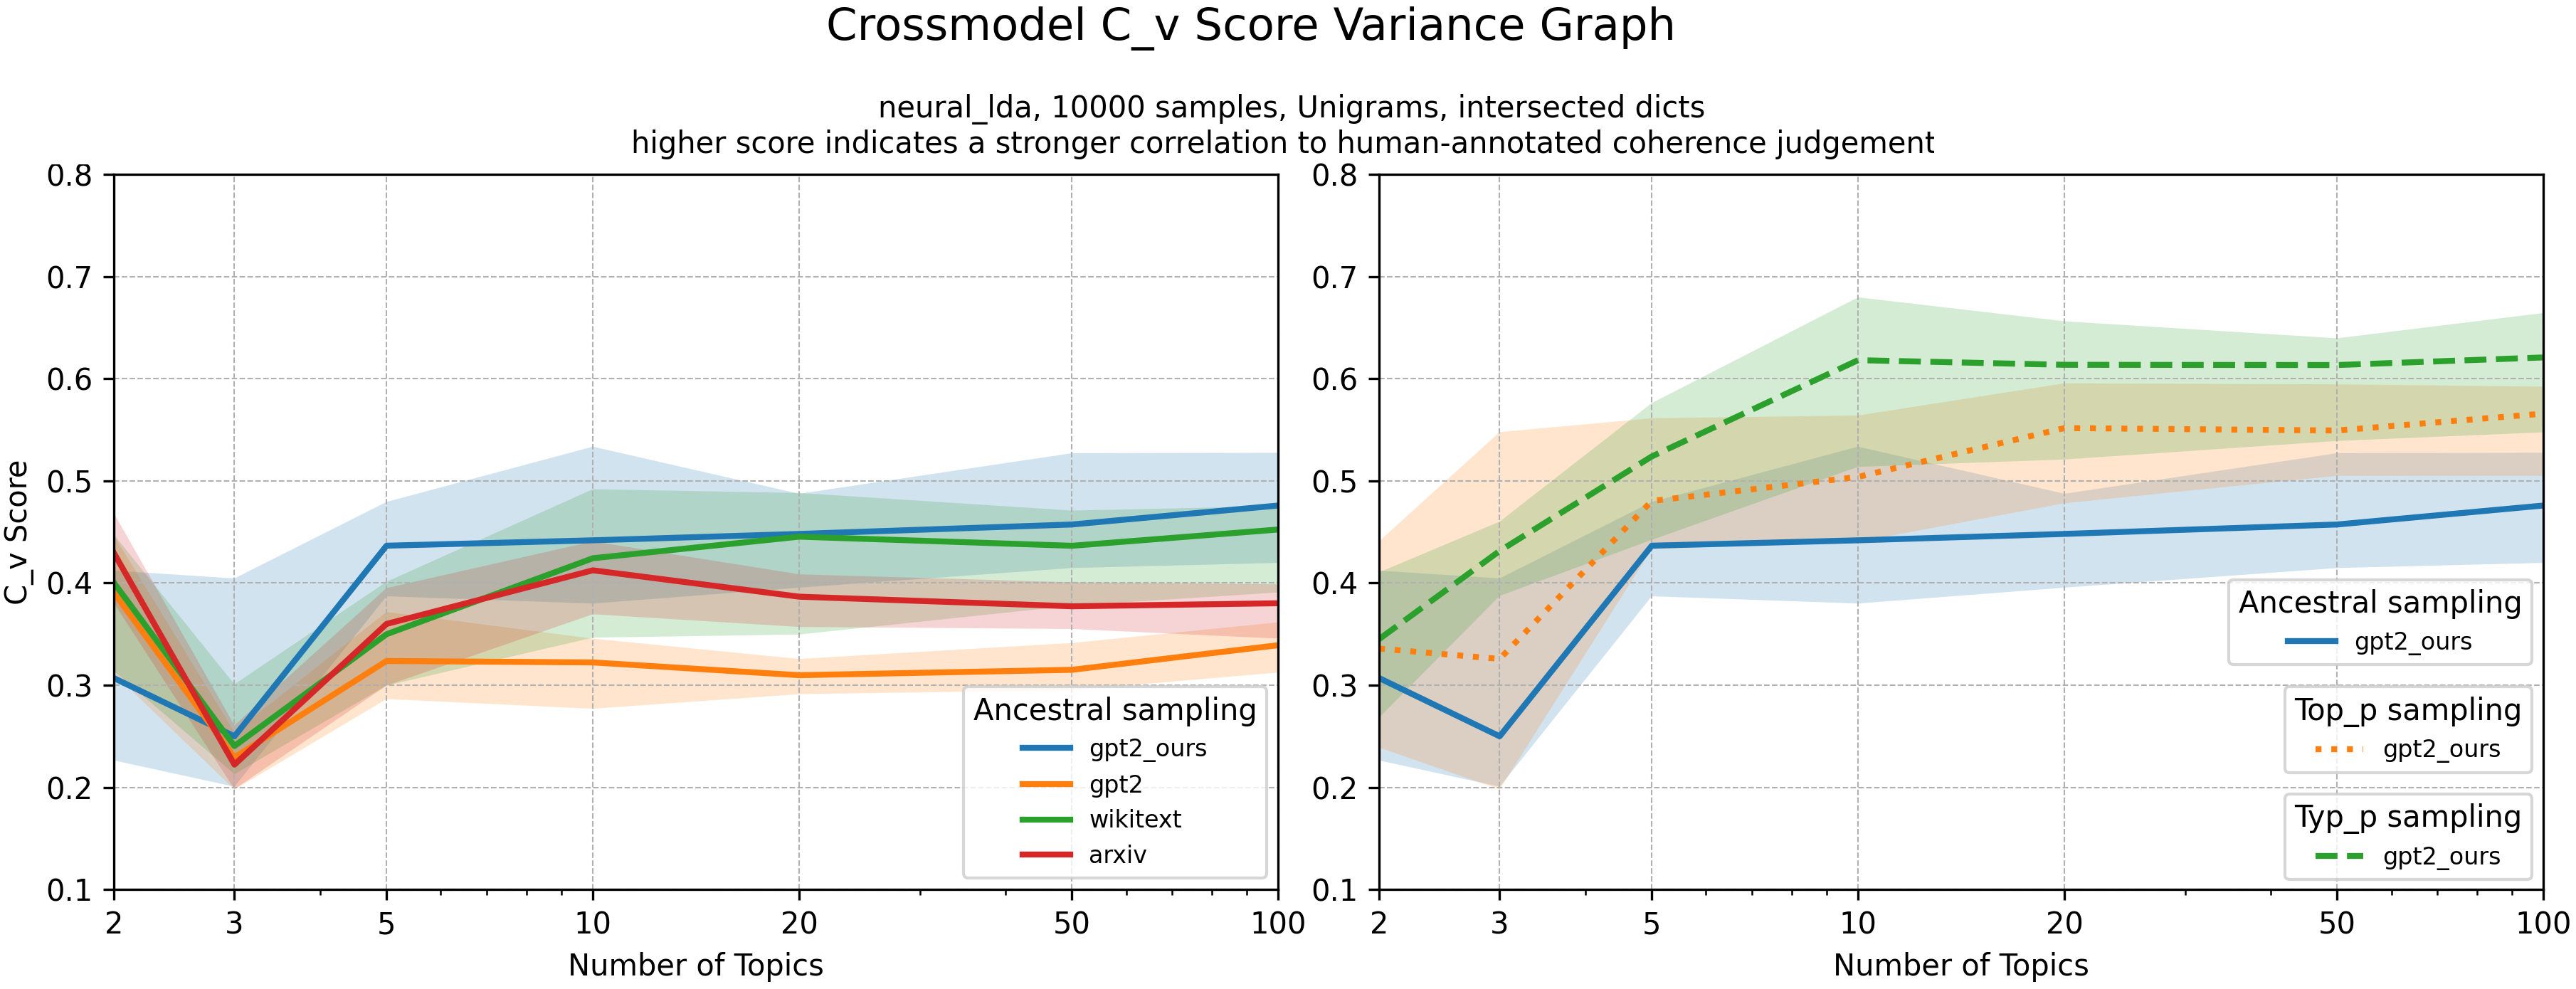
\includegraphics[width=1\textwidth]{figures/Unigrams-10000-crossmodel-cv-var-neural_lda-gpt2+nt-is}
    \caption{Topic coherence of topic models with slightly different dictionaries.}
    \label{fig:Unigrams-10000-crossmodel-cv-var-neural_lda-gpt2+nt-is}
\end{figure}

% =======================================
\subsubsection{Transformer-XL With Neural LDA}
The quality of topic models created with neural LDA in respect to both Transformer-XL models is very similar to the GPT-2 results. In fig. \ref{fig:Unigrams-10000-crossmodel-cv-var-neural_lda-trafo_xl+nt-is} on the left, we see again the peaks at 3 topics. At a topic size of 5 or more, the topic model quality ranges from $0.31$ to $0.51$ with a variance of up to $\pm0.1$. The quality of 5 topics or more is more or less horizontal and on average worse than the classic LDA topic models. 

The quality of neural LDA topic models from the corpus sampled with Typical (and Top-P) sampling is much smoother. Additionally, for 3 topics or more, the quality is improved (see fig. \ref{fig:Unigrams-10000-crossmodel-cv-var-neural_lda-trafo_xl+nt-is} on the right).
\begin{figure}[H]
    \centering
    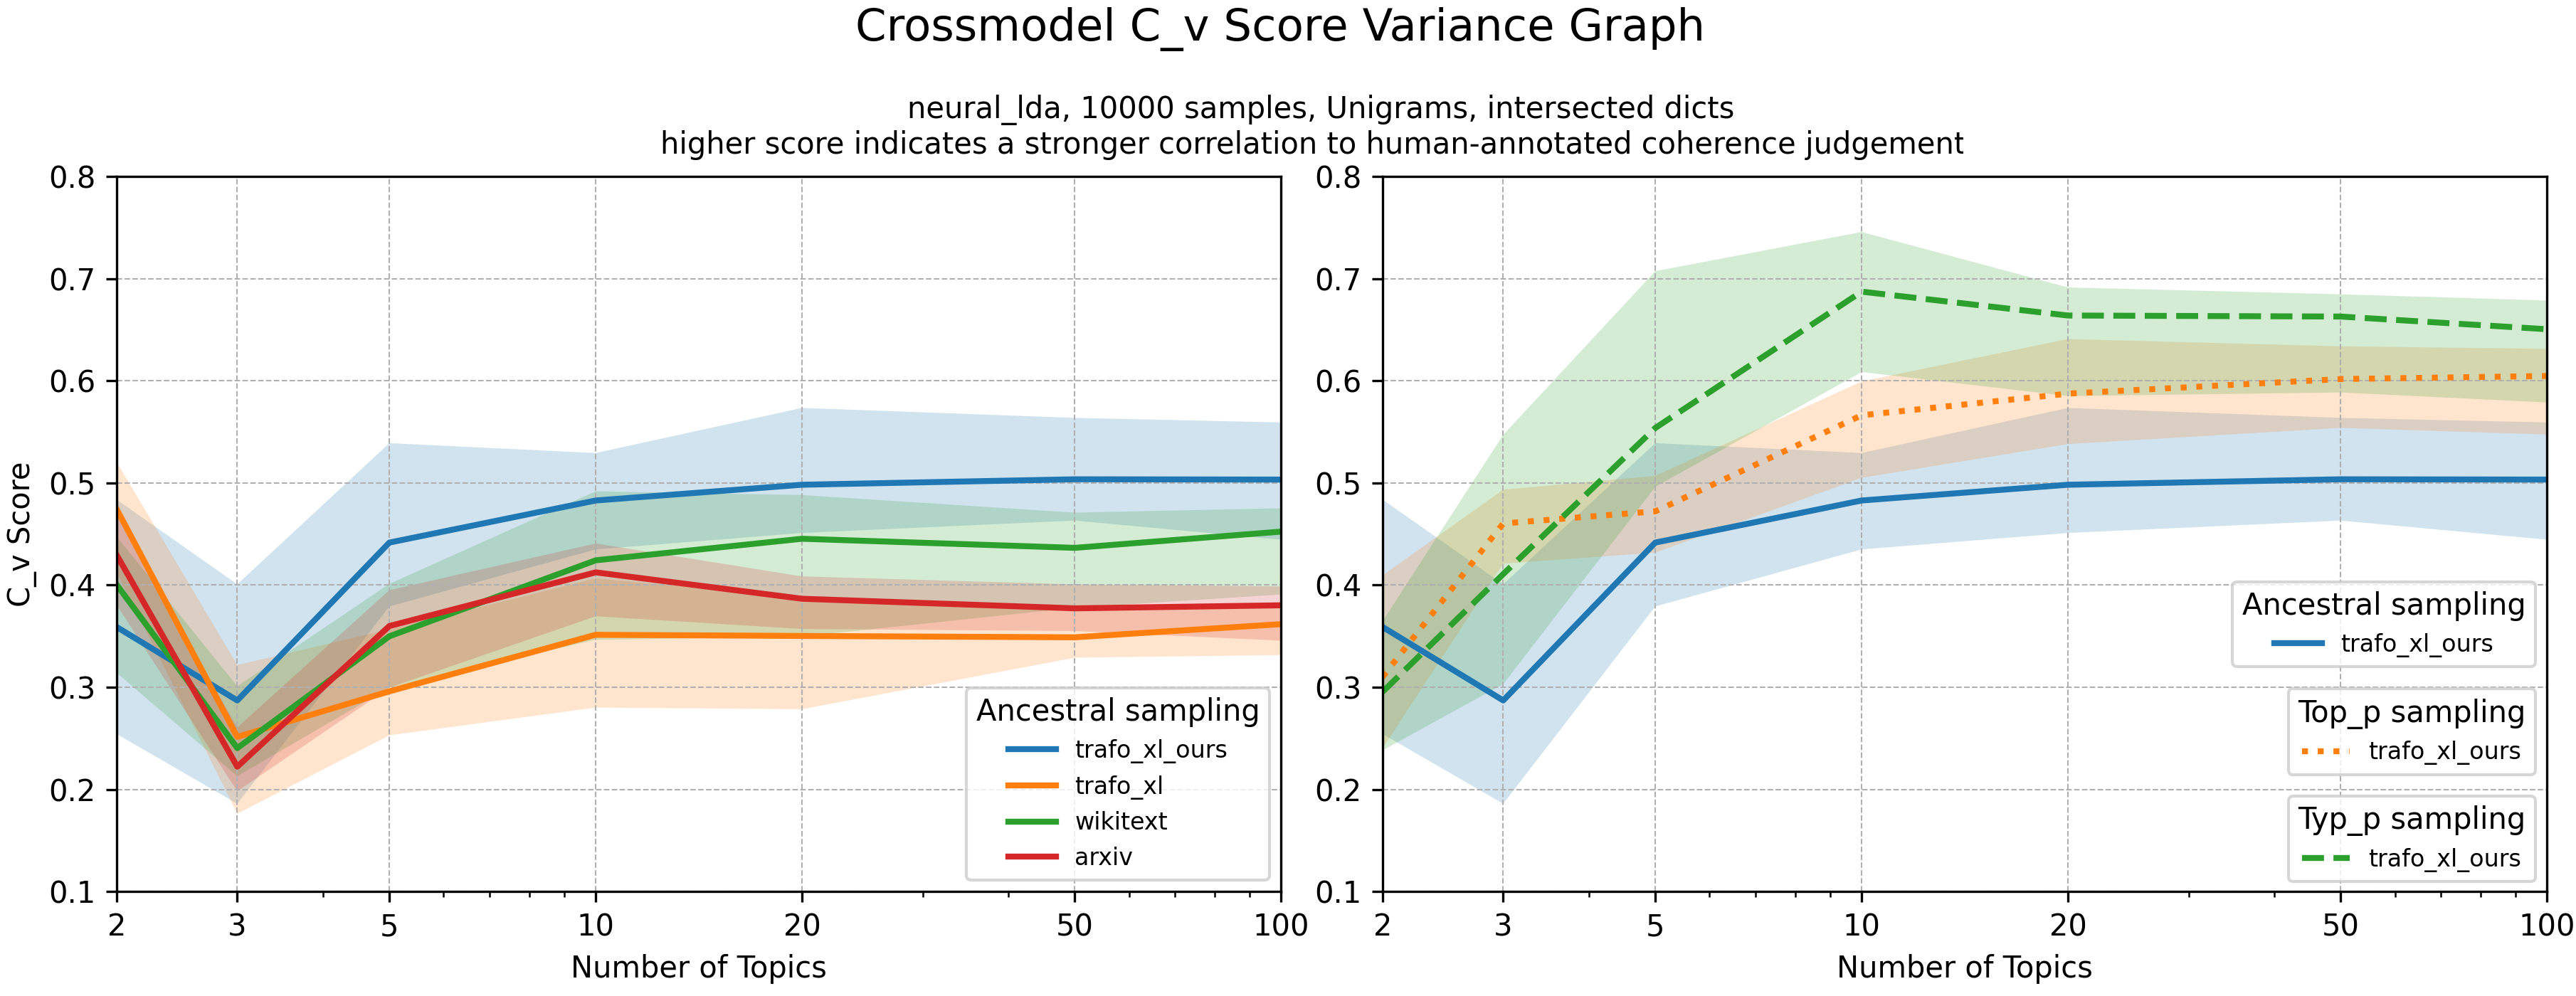
\includegraphics[width=1\textwidth]{figures/Unigrams-10000-crossmodel-cv-var-neural_lda-trafo_xl+nt-is}
    \caption{Topic coherence of topic models with slightly different dictionaries.}
    \label{fig:Unigrams-10000-crossmodel-cv-var-neural_lda-trafo_xl+nt-is}
\end{figure}


% =======================================
\subsection{Variance of Our Metric for Comparing Topic Models}
To be able to make some assumptions about our final results with a certain degree of confidence, we measure the variance of our metric on the following topic model comparisons for 100'000 and 10'000 documents: \texttt{gpt2\_ours} vs. \texttt{gpt2\_ours}, \texttt{gpt2\_ours} vs. \texttt{wikitext} and \texttt{gpt2\_ours} vs. \texttt{arxiv}.

Fig. \ref{fig:Unigrams-var-tt-is} shows that for topic models with a higher number of topics, especially for corpora with 100'000 documents (graph on the left), the metric tends to be stable in respect to variance. The variance for topic models from corpora with 100'000 documents collapses nearly to 0 for a higher number of topics. Topic models from corpora with 10'000 documents tend to have a slightly higher variance of up to $\pm0.1$.  
\begin{figure}[H]
    \centering
    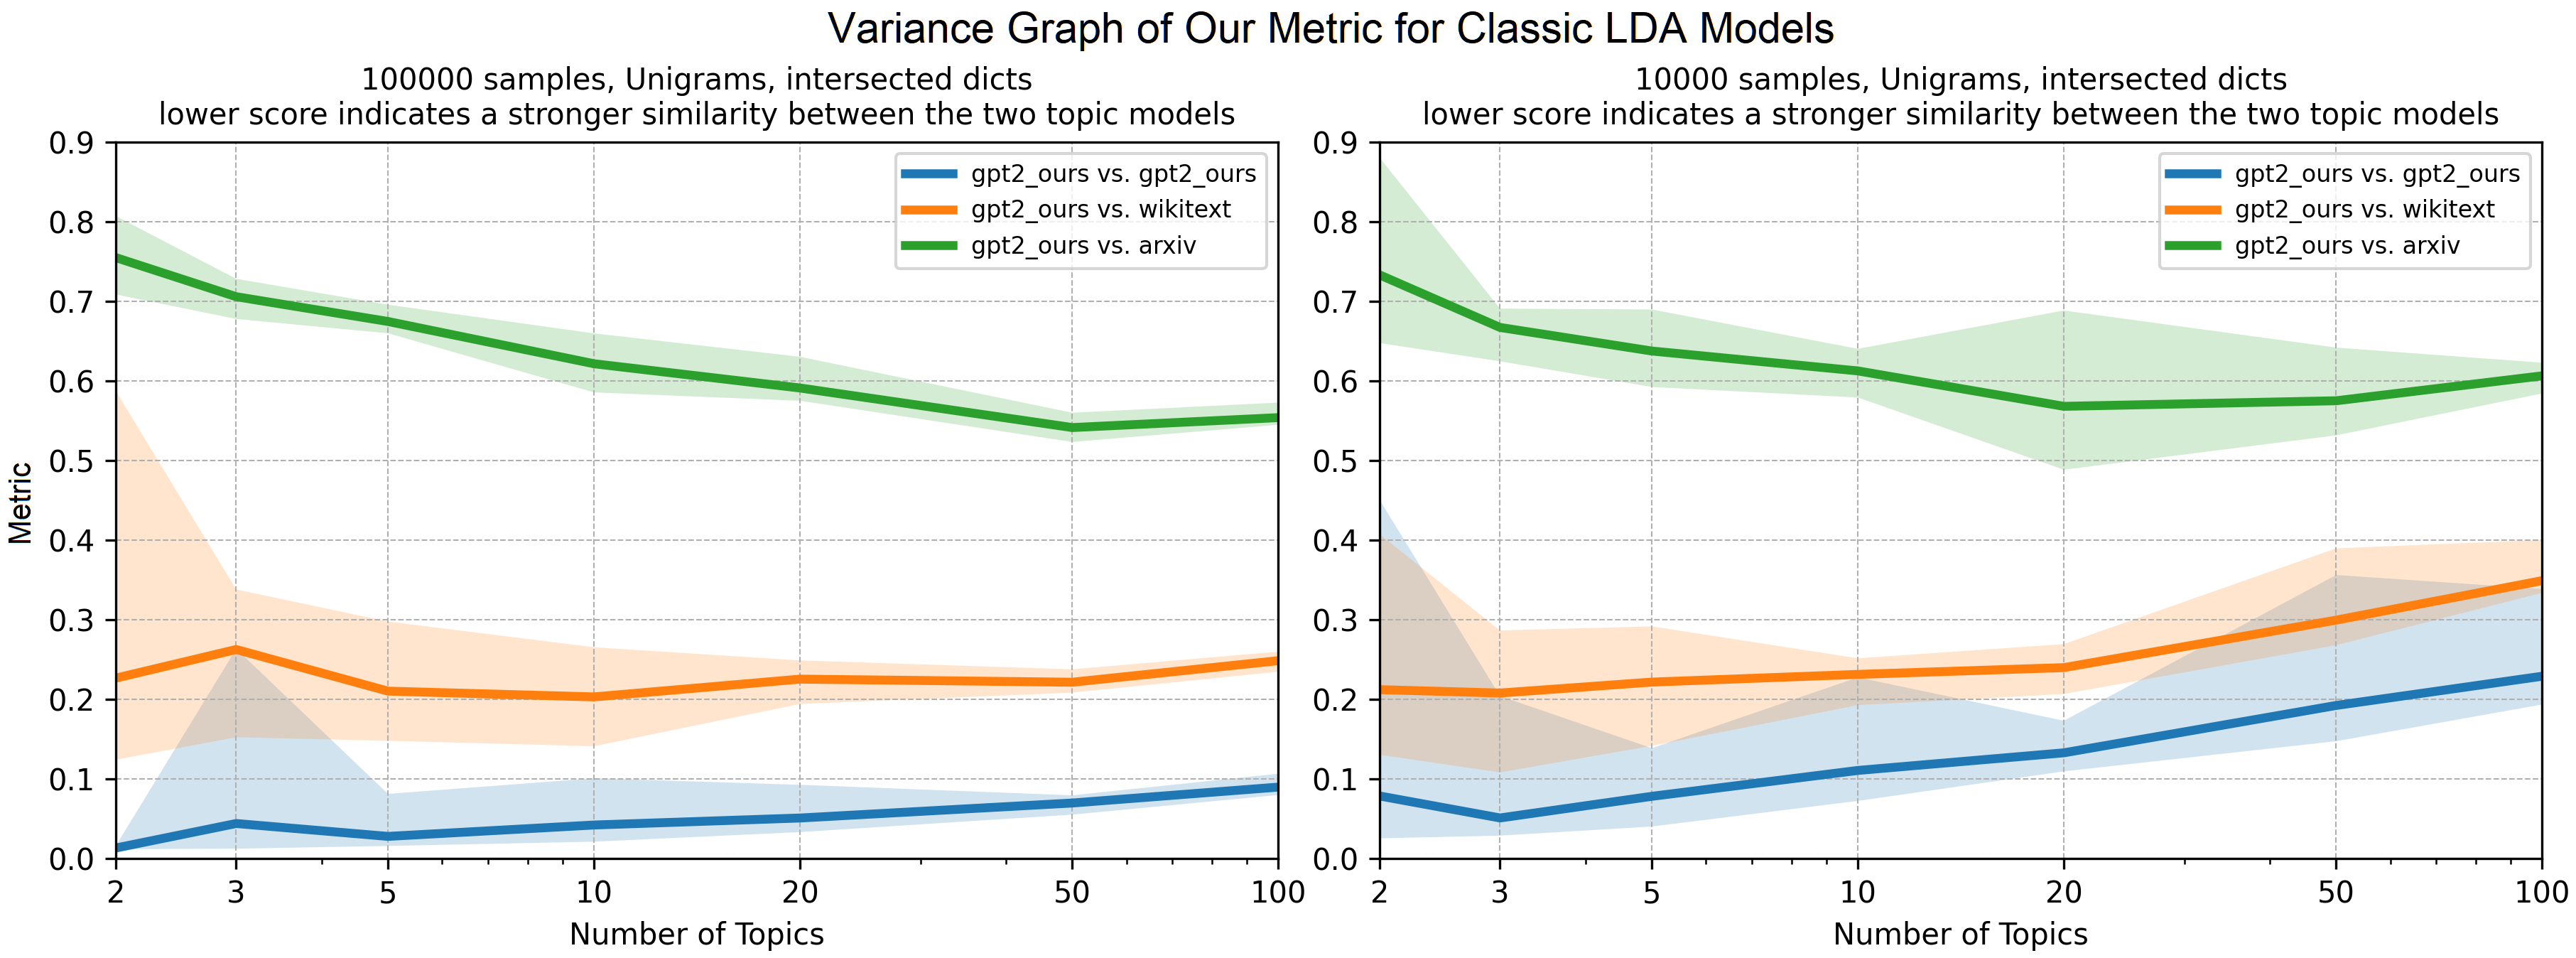
\includegraphics[width=1\textwidth]{figures/Unigrams-var-tt-is}
    \caption{Variance of the topic model comparison metric for corpora with 100'000 and 10'000 samples.}
    \label{fig:Unigrams-var-tt-is}
\end{figure}

% =======================================
\subsection{Comparisons of Our Topic Models}\label{sec:comp}
In order to make some assumptions about our findings, we need a baseline. Specifically, we need to know what it means to compare two similar topic models and what it means to compare two dissimilar topic models in respect to our metric. 

To find an upper boundary for the area of similar topic models, we compare topic models from the same corpus, i.e. \texttt{dataset1-*} vs. \texttt{dataset2-*}. To find a lower boundary for the area of different topic models, we compare topic models from corpora we know are different, i.e. \texttt{wikitext} vs. \texttt{arxiv}.

% =======================================
\subsubsection{Corpora With 100'000 Documents}
For corpora with 100'000 documents (see fig. \ref{fig:Unigrams-100000-crossmodel-tt-gpt2-classic_lda-ab-is} on the left), the \texttt{arxiv} corpus compared to other corpora results in a value of greater than $0.52$. When comparing topic models from the same corpora, the value is below $0.2$. The comparisons between topic models from corpora \texttt{gpt2\_ours}, \texttt{gp2} and \texttt{wikitext} result in a value ranging from $0.2$ and $0.52$.

In contrast to the improvement in quality of our topic models with help of other sampling methods, we cannot say the same in regard to our comparison metric. In fig. \ref{fig:Unigrams-100000-crossmodel-tt-gpt2-classic_lda-ab-is} on the right, we cannot see a general improvement of our metric values when using Typical or Top-P sampling. Instead, in some occasions (dashed red line vs. red line), the topic models differ clearly from each other. 
\begin{figure}[H]
    \centering
    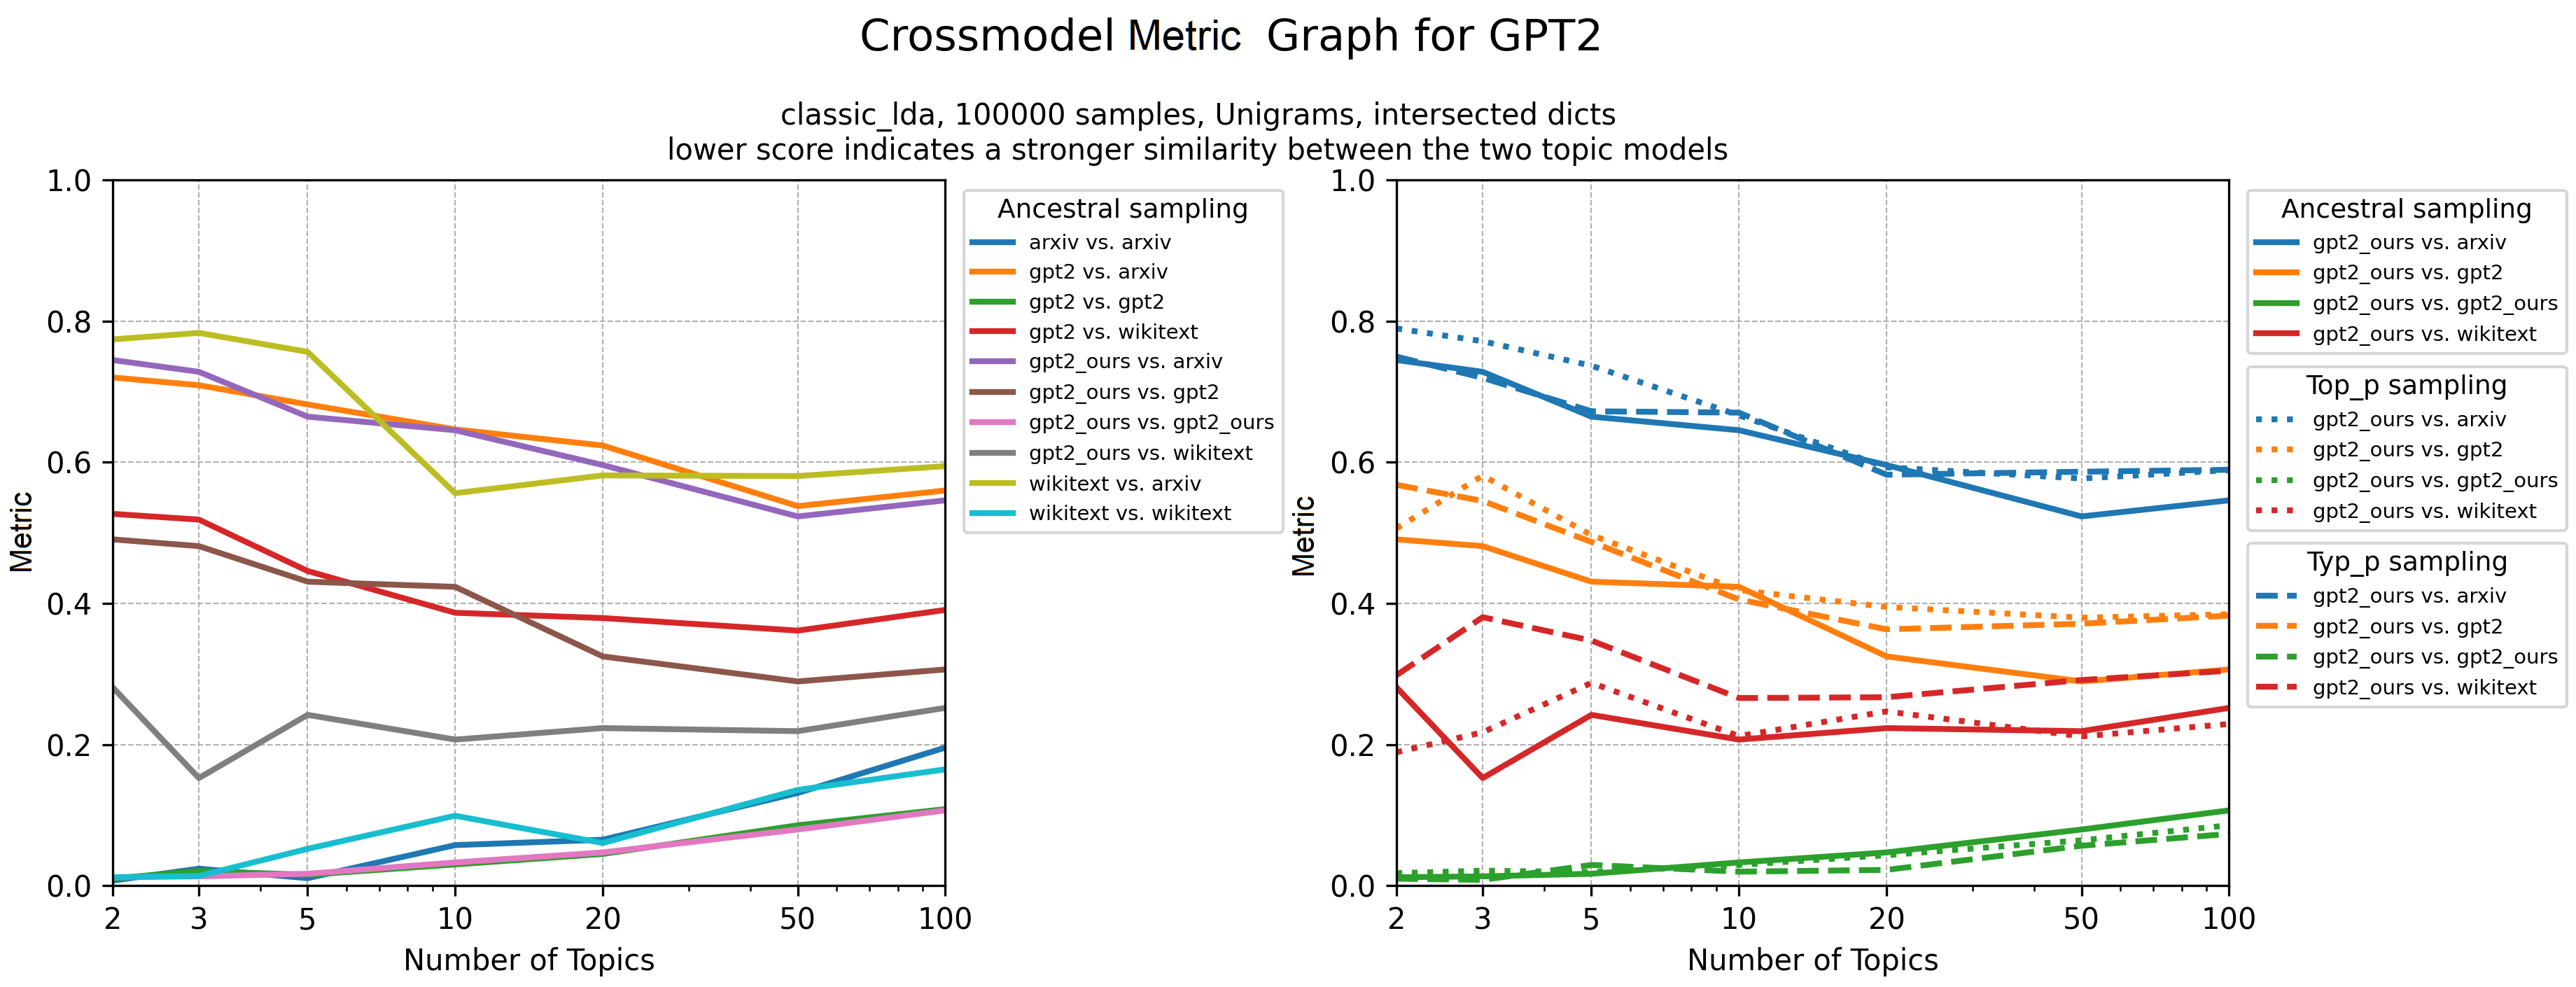
\includegraphics[width=1\textwidth]{figures/Unigrams-100000-crossmodel-tt-gpt2-classic_lda-ab-is}
    \caption{Topic model comparison metric (GPT-2, classic LDA, 100'000 samples).}
    \label{fig:Unigrams-100000-crossmodel-tt-gpt2-classic_lda-ab-is}
\end{figure}

% =======================================
\subsubsection{Corpora With 10'000 Documents}
% =======================================
\subsubsection{GPT-2 and Classic LDA}
For corpora with 10'000 documents in respect to GPT-2 and topic models created with classic LDA (see fig. \ref{fig:Unigrams-10000-crossmodel-tt-gpt2-classic_lda-ab-is} on the left), the \texttt{arxiv} corpus compared to other corpora results in a value of greater than $0.5$. When comparing topic models from the same corpora, the value is below $0.2$. For topic sizes of up to 20 topics, the value is below $0.4$. The comparisons between topic models from corpora \texttt{gpt2\_ours} and \texttt{wikitext} result in a value ranging from $0.14$ to $0.32$.

In contrast to the topic model quality measurements, other sampling methods do not seem to improve our comparison metric. In fig. \ref{fig:Unigrams-10000-crossmodel-tt-gpt2-classic_lda-ab-is} on the right, we cannot see a general improvement of our values when using Typical or Top-P sampling. Instead, in some occasions (dashed red line vs. red line), the topic models differ clearly from each other.
\begin{figure}[H]
    \centering
    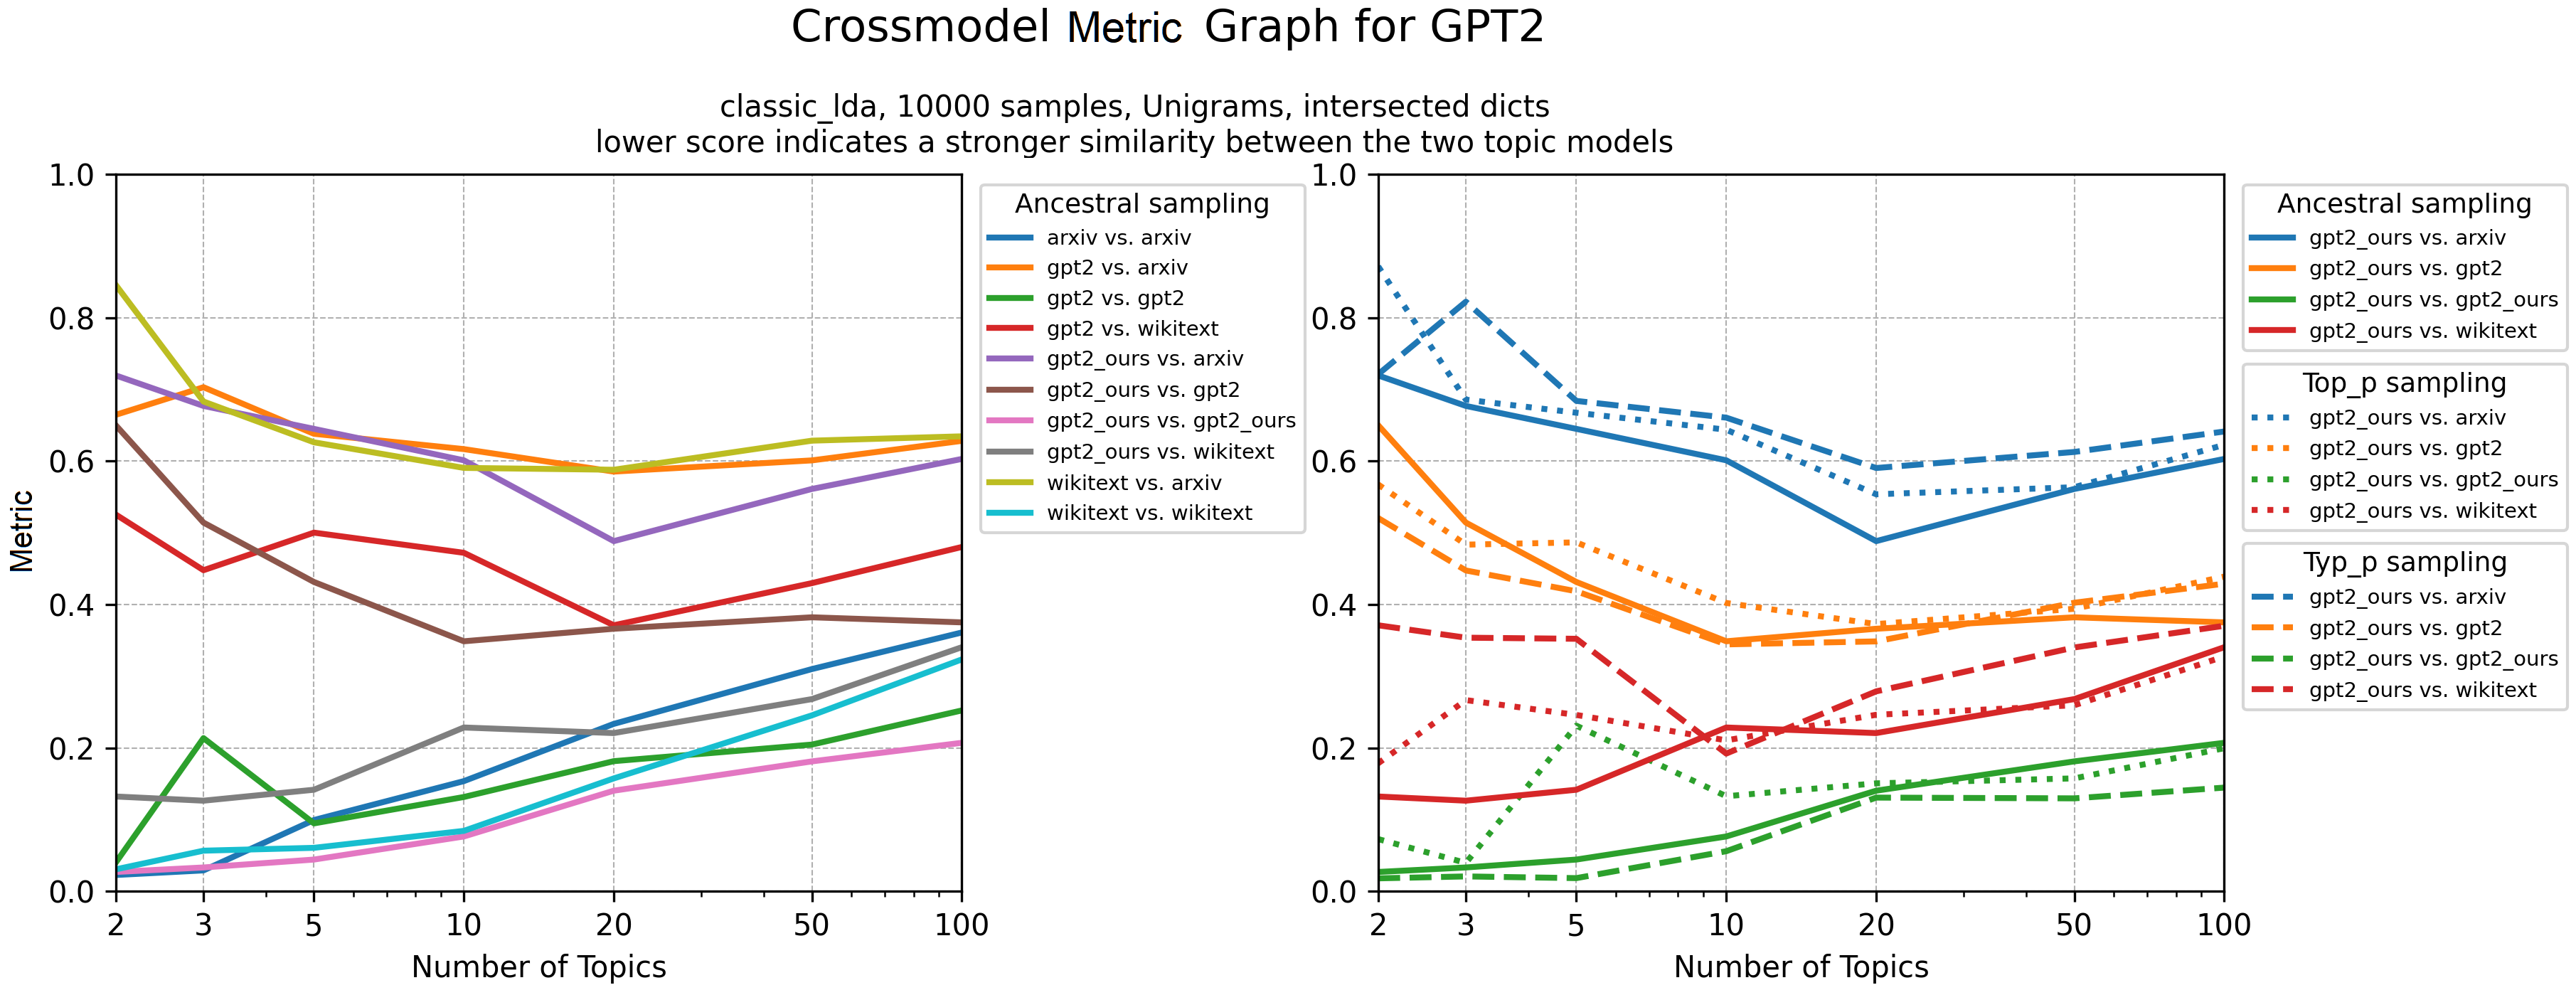
\includegraphics[width=1\textwidth]{figures/Unigrams-10000-crossmodel-tt-gpt2-classic_lda-ab-is}
    \caption{Topic model comparison score (GPT-2, classic LDA, 10'000 samples).}
    \label{fig:Unigrams-10000-crossmodel-tt-gpt2-classic_lda-ab-is}
\end{figure}

% =======================================
\subsubsection{Transformer-XL and Classic LDA}
For the results in respect to Transformer-XL and topic models created with classic LDA (see fig. \ref{fig:Unigrams-10000-crossmodel-tt-trafo_xl-classic_lda-ab-is} on the left), the \texttt{arxiv} corpus compared to other corpora results in a value above $0.6$. When comparing topic models from the same corpora, the upper boundary is linearly increasing from $0.2$ for topic size 2 up to $0.45$ for topic size 100. The comparisons between topic models from corpora \texttt{trafo\_xl\_ours} and \texttt{wikitext} result in a value slightly lower than the upper boundary from the area of similarity.

Other sampling methods have various impacts on our results. In fig. \ref{fig:Unigrams-10000-crossmodel-tt-trafo_xl-classic_lda-ab-is} on the right, we can see an improvement when comparing two nearly identical topic models (green line vs. green dashed/dotted line). For all other comparisons, there is no general improvement when using Typical or Top-P sampling.
\begin{figure}[H]
    \centering
    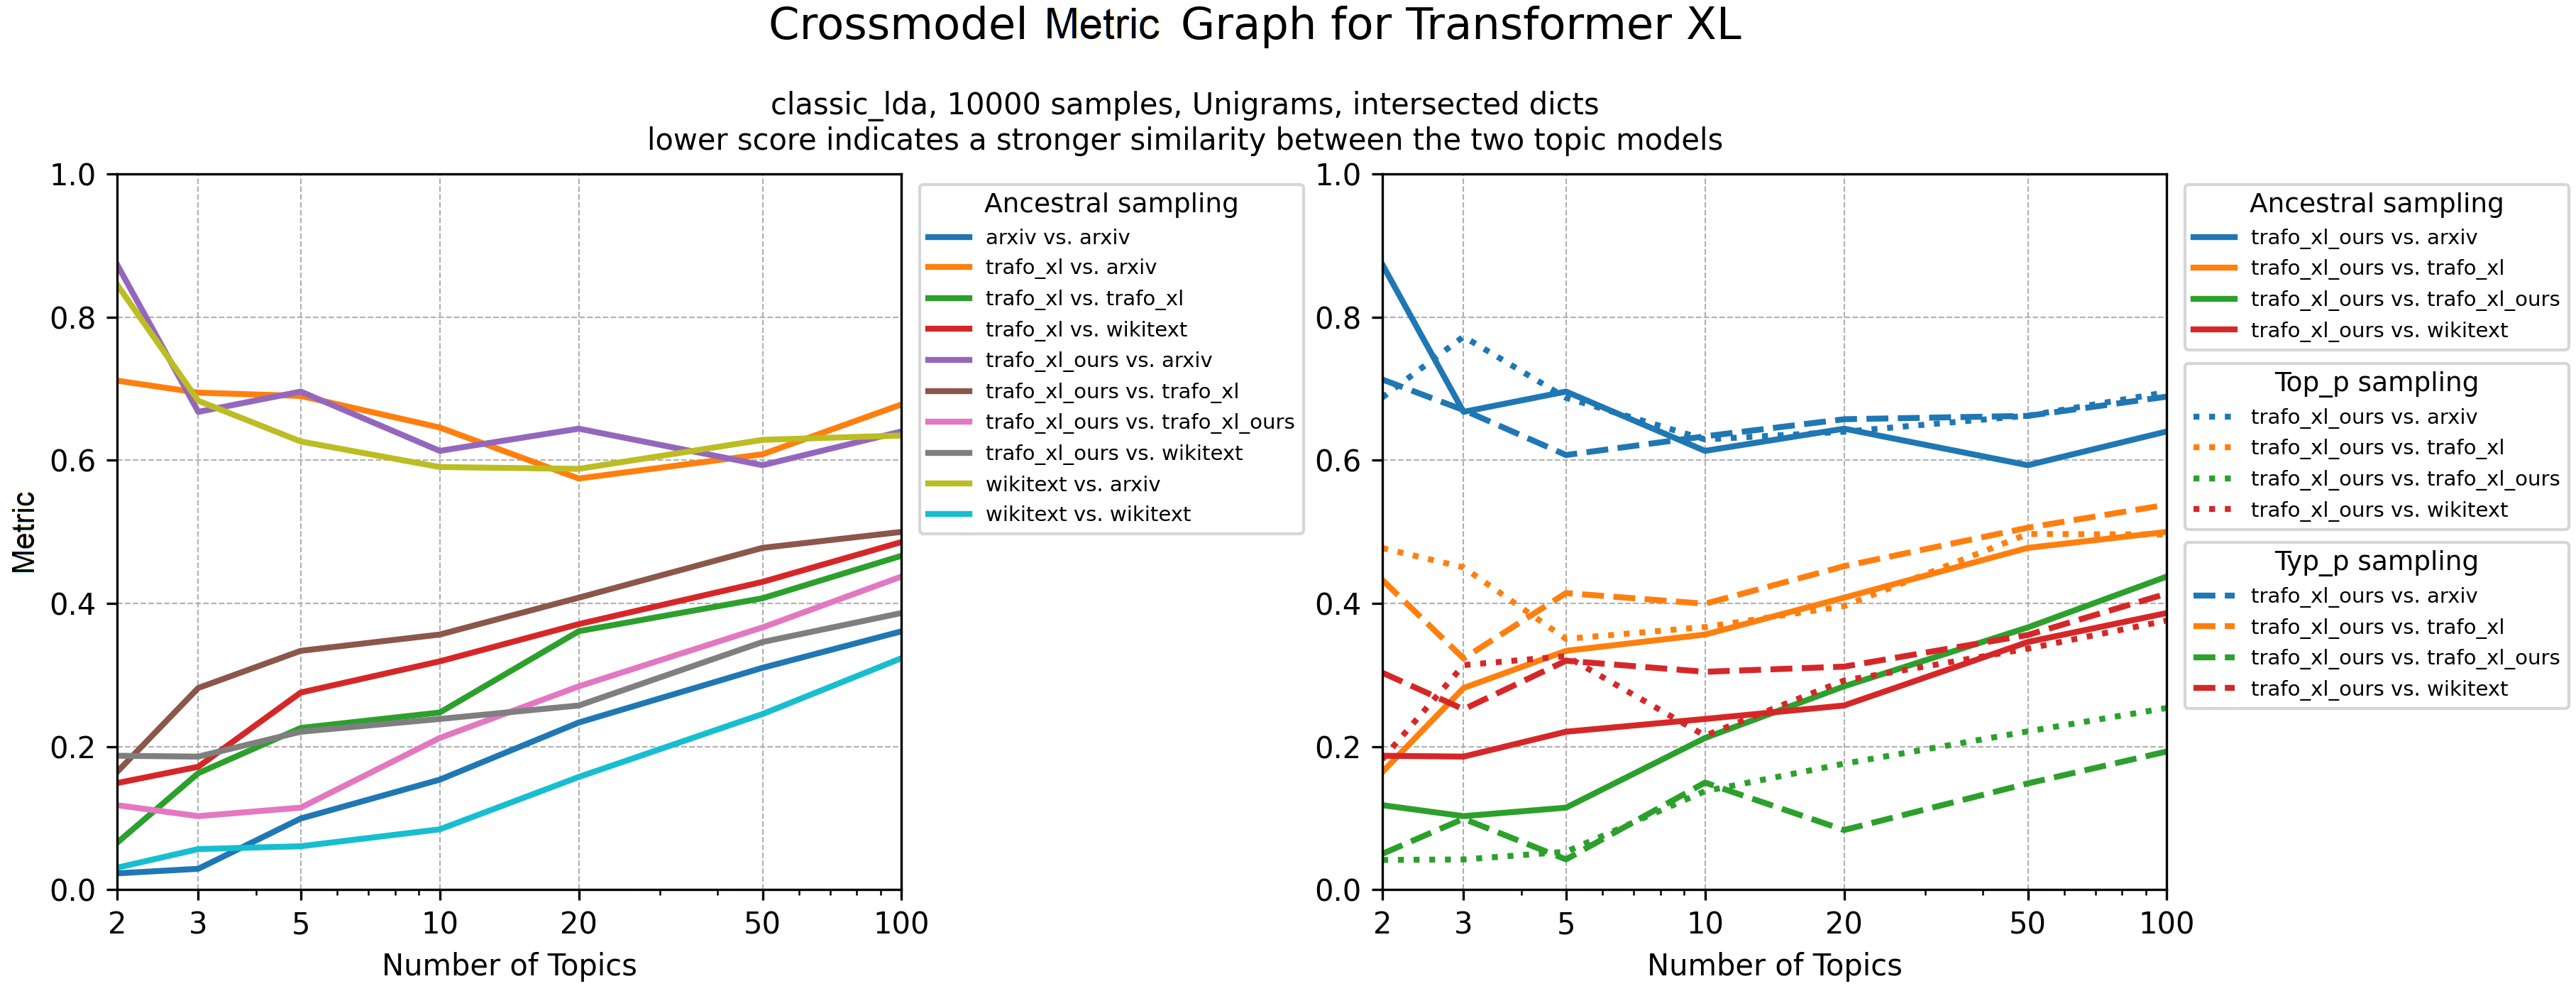
\includegraphics[width=1\textwidth]{figures/Unigrams-10000-crossmodel-tt-trafo_xl-classic_lda-ab-is}
    \caption{Topic model comparison metric (Transformer-XL, classic LDA, 10'000 samples).}
    \label{fig:Unigrams-10000-crossmodel-tt-trafo_xl-classic_lda-ab-is}
\end{figure}

% =======================================
\subsubsection{GPT-2 and Neural LDA}
In the results for GPT-2 and topic models created with neural LDA (see \ref{fig:Unigrams-10000-crossmodel-tt-gpt2-neural_lda-ab-is} on the left), we find some similar tendencies as in the data from before. The \texttt{arxiv} corpus compared to other corpora results in a value above $0.53$. When comparing topic models from the same corpora, the upper boundary is generally increasing from $0.1$ for a topic size of 2 up to $0.45$ for a topic size of 100. The results of the comparisons between topic models from corpora \texttt{gpt2\_ours} and \texttt{wikitext} fall into the area of similarity, except for 2 topics. There we can see a distinctive difference.

Other sampling methods have few impacts on our results. In fig. \ref{fig:Unigrams-10000-crossmodel-tt-gpt2-neural_lda-ab-is} on the right, we can see no improvements in general which could not be related to variance. The comparison between \texttt{gpt2\_ours} and \texttt{wikitext} is an exemption. There it is clearly visible that Typical sampling has an impact on the smoothness of the curve (red line vs. red dashed line).  
\begin{figure}[H]
    \centering
    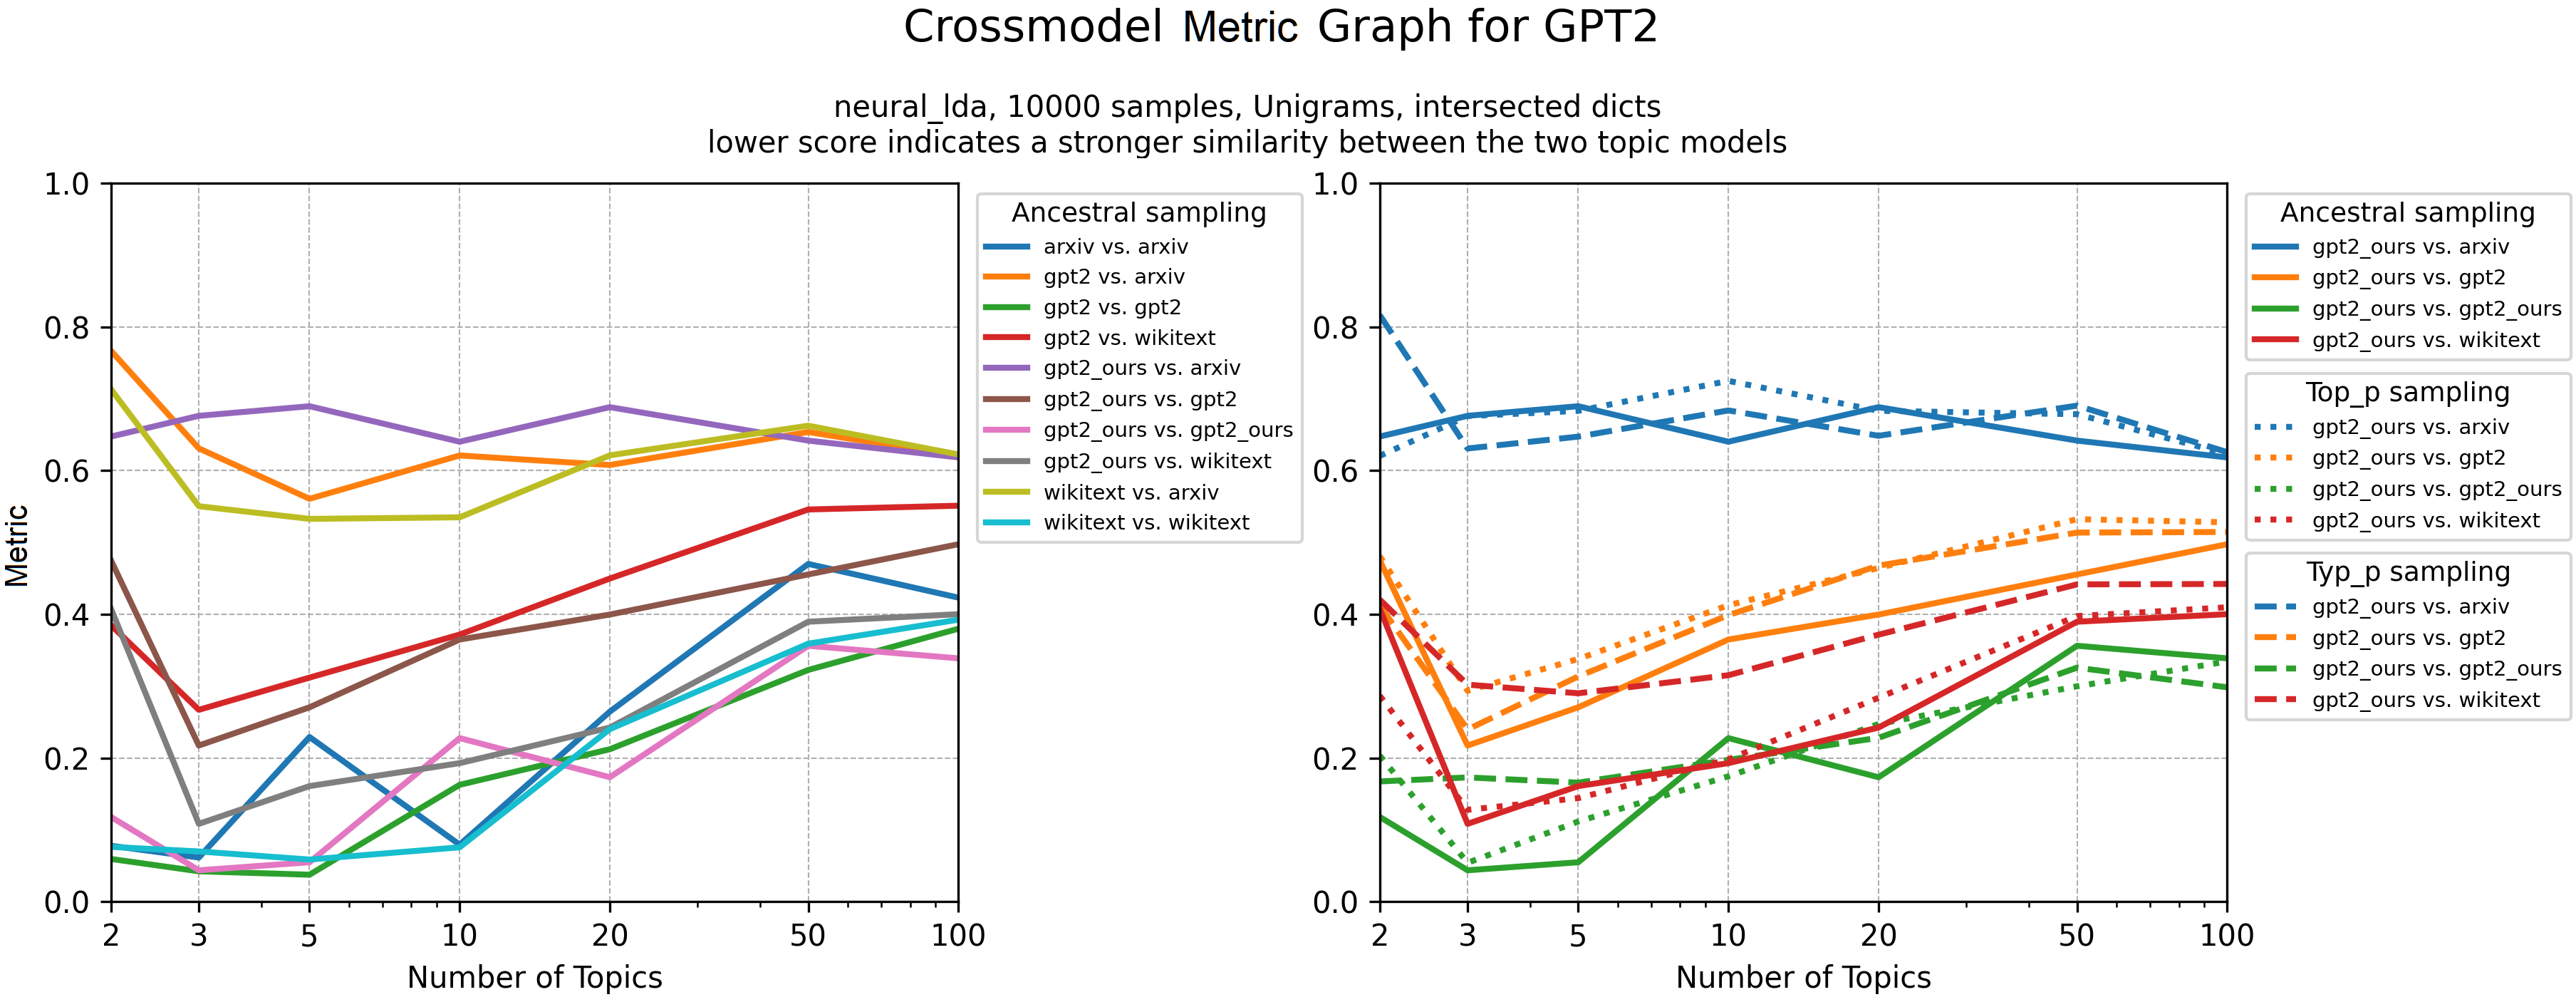
\includegraphics[width=1\textwidth]{figures/Unigrams-10000-crossmodel-tt-gpt2-neural_lda-ab-is}
    \caption{Topic model comparison metric (GPT-2, neural LDA, 10'000 samples).}
    \label{fig:Unigrams-10000-crossmodel-tt-gpt2-neural_lda-ab-is}
\end{figure}

% =======================================
\subsubsection{Transformer-XL and Neural LDA}
In the results for Transformer-XL and topic models created with neural LDA (see \ref{fig:Unigrams-10000-crossmodel-tt-trafo_xl-neural_lda-ab-is} on the left), we find the same tendencies as with the results for GPT-2 topic models created with neural LDA. The \texttt{arxiv} corpus compared to other corpora results in a value above $0.5$ and when comparing topic models from the same corpora, the upper boundary is generally increasing from $0.2$ for a topic size of 2 up to $0.5$ for a topic size of 100. The results of the comparisons between topic models from corpora \texttt{trafo\_xl\_ours} and \texttt{wikitext} fall into the area of similarity, except for 2 topics. There we can see a distinctive difference once again.

Other sampling methods have a rather chaotic impact on some of our results. In fig. \ref{fig:Unigrams-10000-crossmodel-tt-trafo_xl-neural_lda-ab-is} on the right, we can see no impact on the comparison with the topic models from \texttt{arxiv} (the blue lines) but a rather chaotic impact on the comparison of \texttt{trafo\_xl\_ours} with itself (the green lines). The comparison between \texttt{trafo\_xl\_ours} and \texttt{wikitext} (the red lines) shows a kind of smoothing of the metric line when comparing ancestral sampling with Top-P sampling and then with Typical sampling. 
\begin{figure}[H]
    \centering
    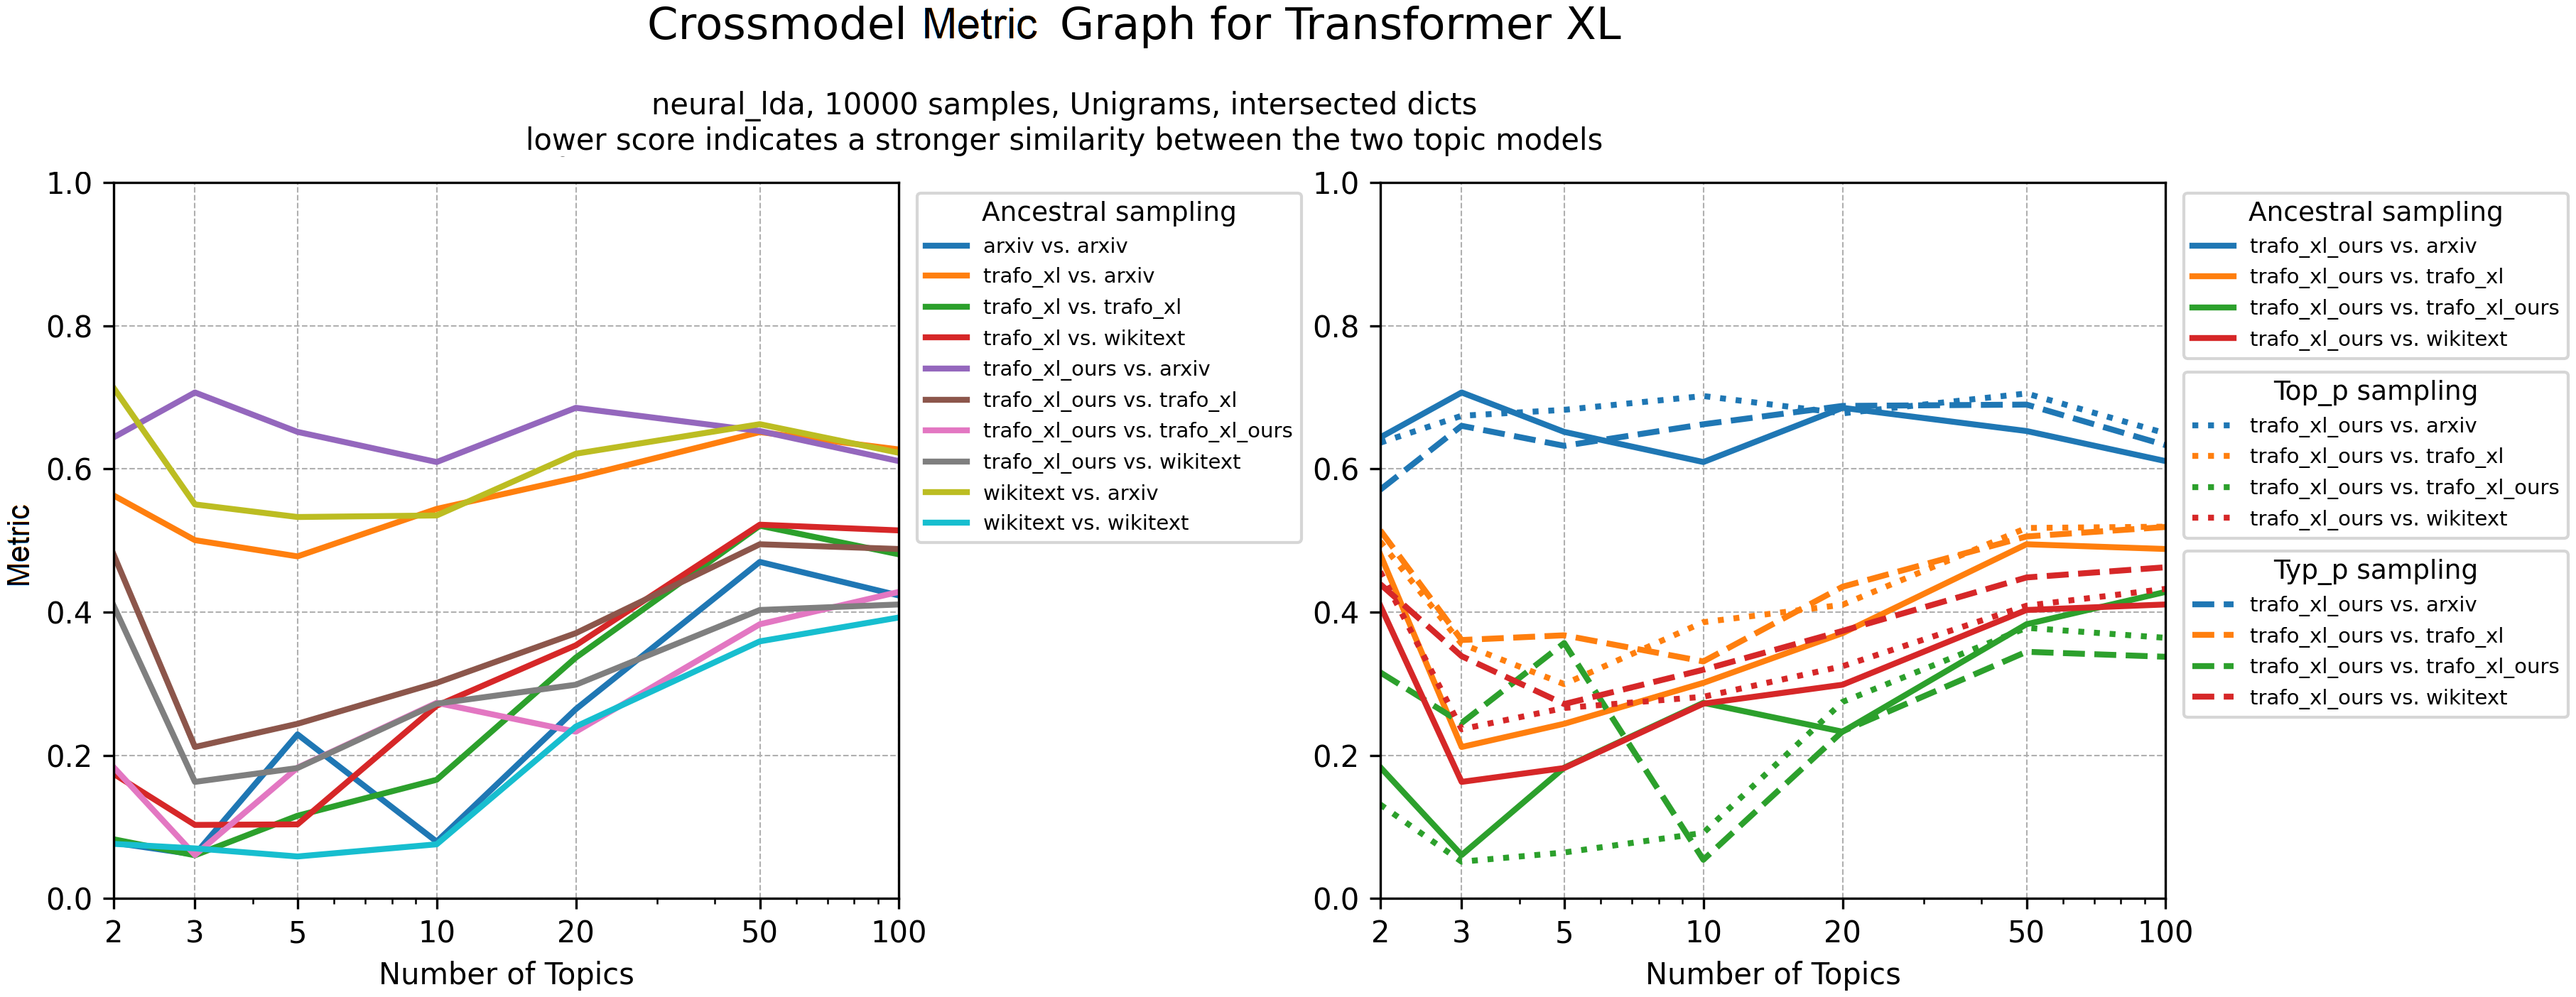
\includegraphics[width=1\textwidth]{figures/Unigrams-10000-crossmodel-tt-trafo_xl-neural_lda-ab-is}
    \caption{Topic model comparison metric (Transformer-XL, neural LDA, 10'000 samples).}
    \label{fig:Unigrams-10000-crossmodel-tt-trafo_xl-neural_lda-ab-is}
\end{figure}
